\newpage
\section{Problem5.9}
\subsection{Rosenbrock函数图像}
首先画出Rosenbrock函数的图像及等值线如下\footnote{由于Rosenbrock函数过于陡峭,因此对原函数进行了取对数处理,以便于观察其特点。}:


\begin{figure}[H]
\centering
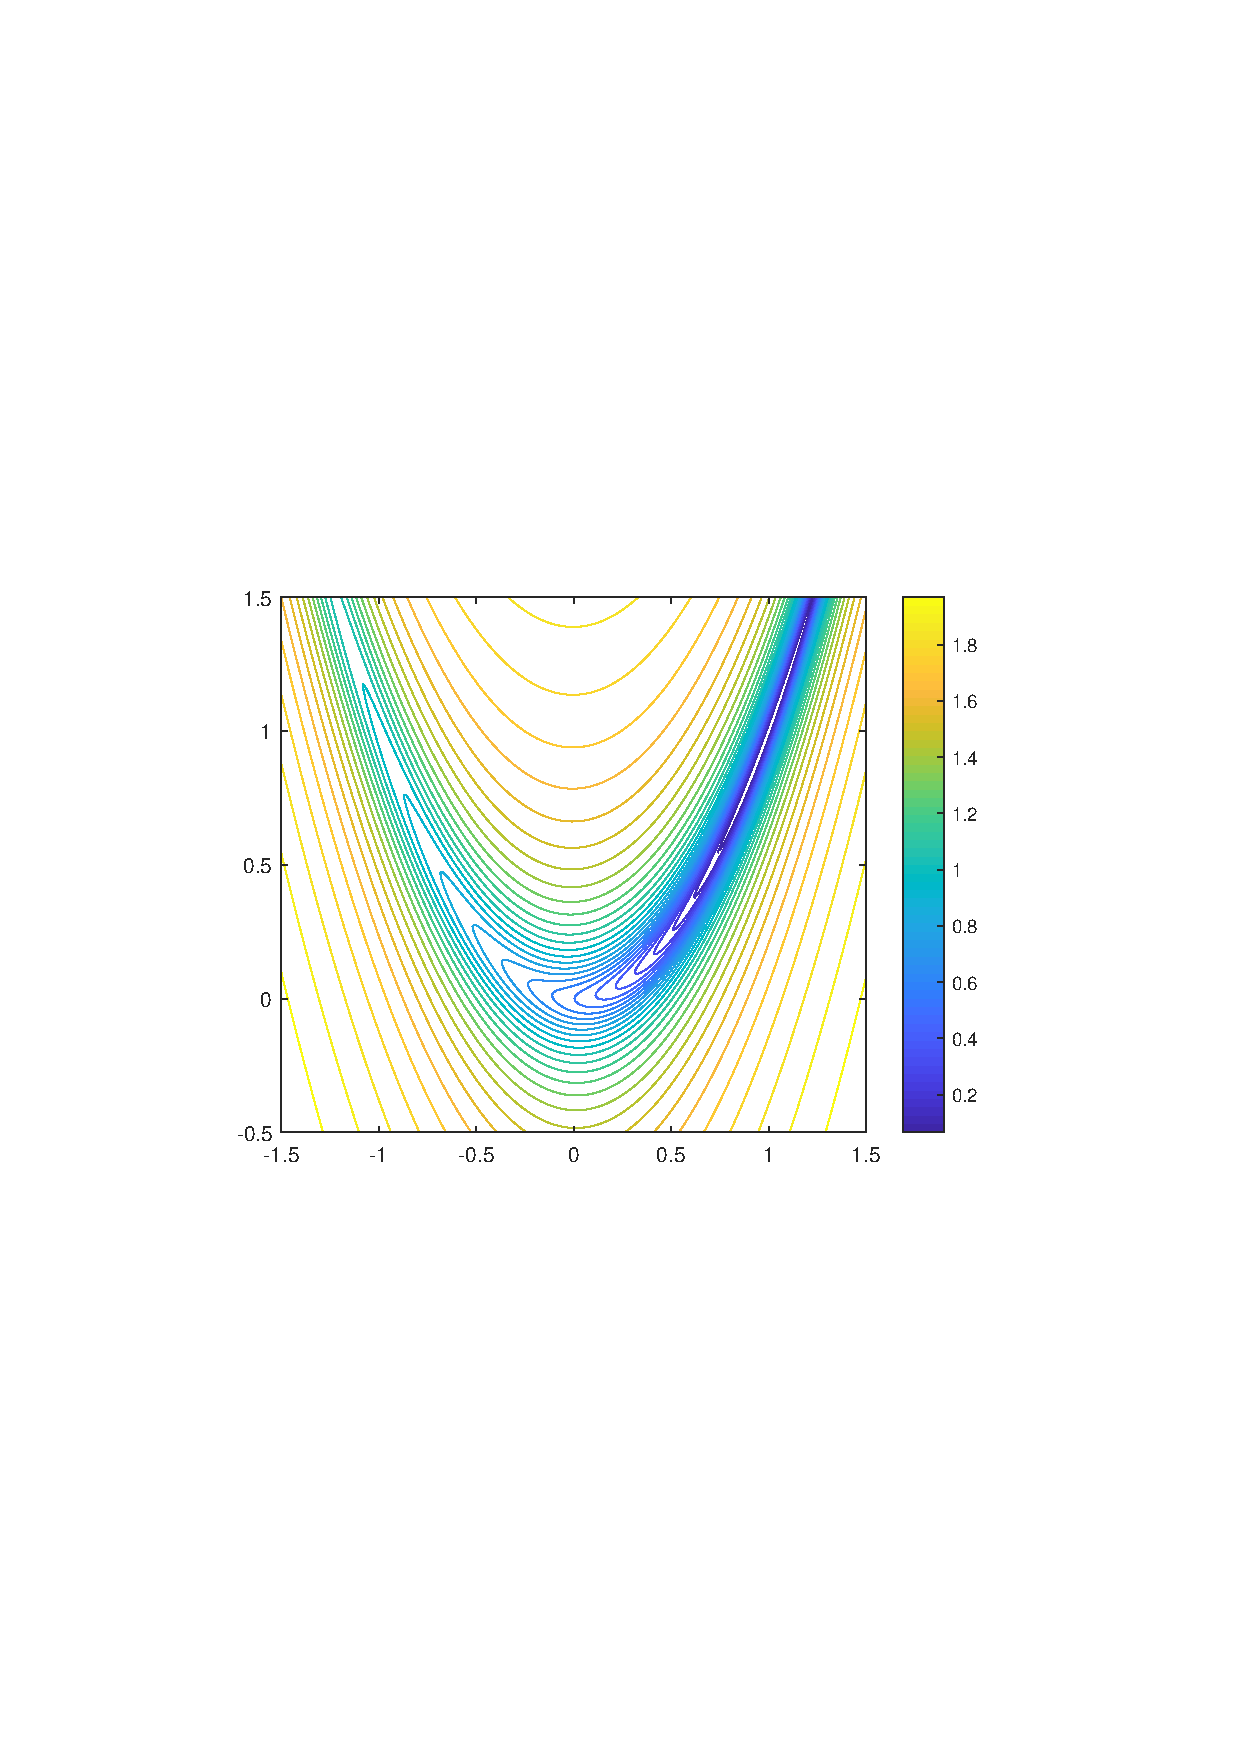
\includegraphics[width=11cm]{fig/4_01.pdf}
\end{figure}


\begin{figure}[H]
\centering
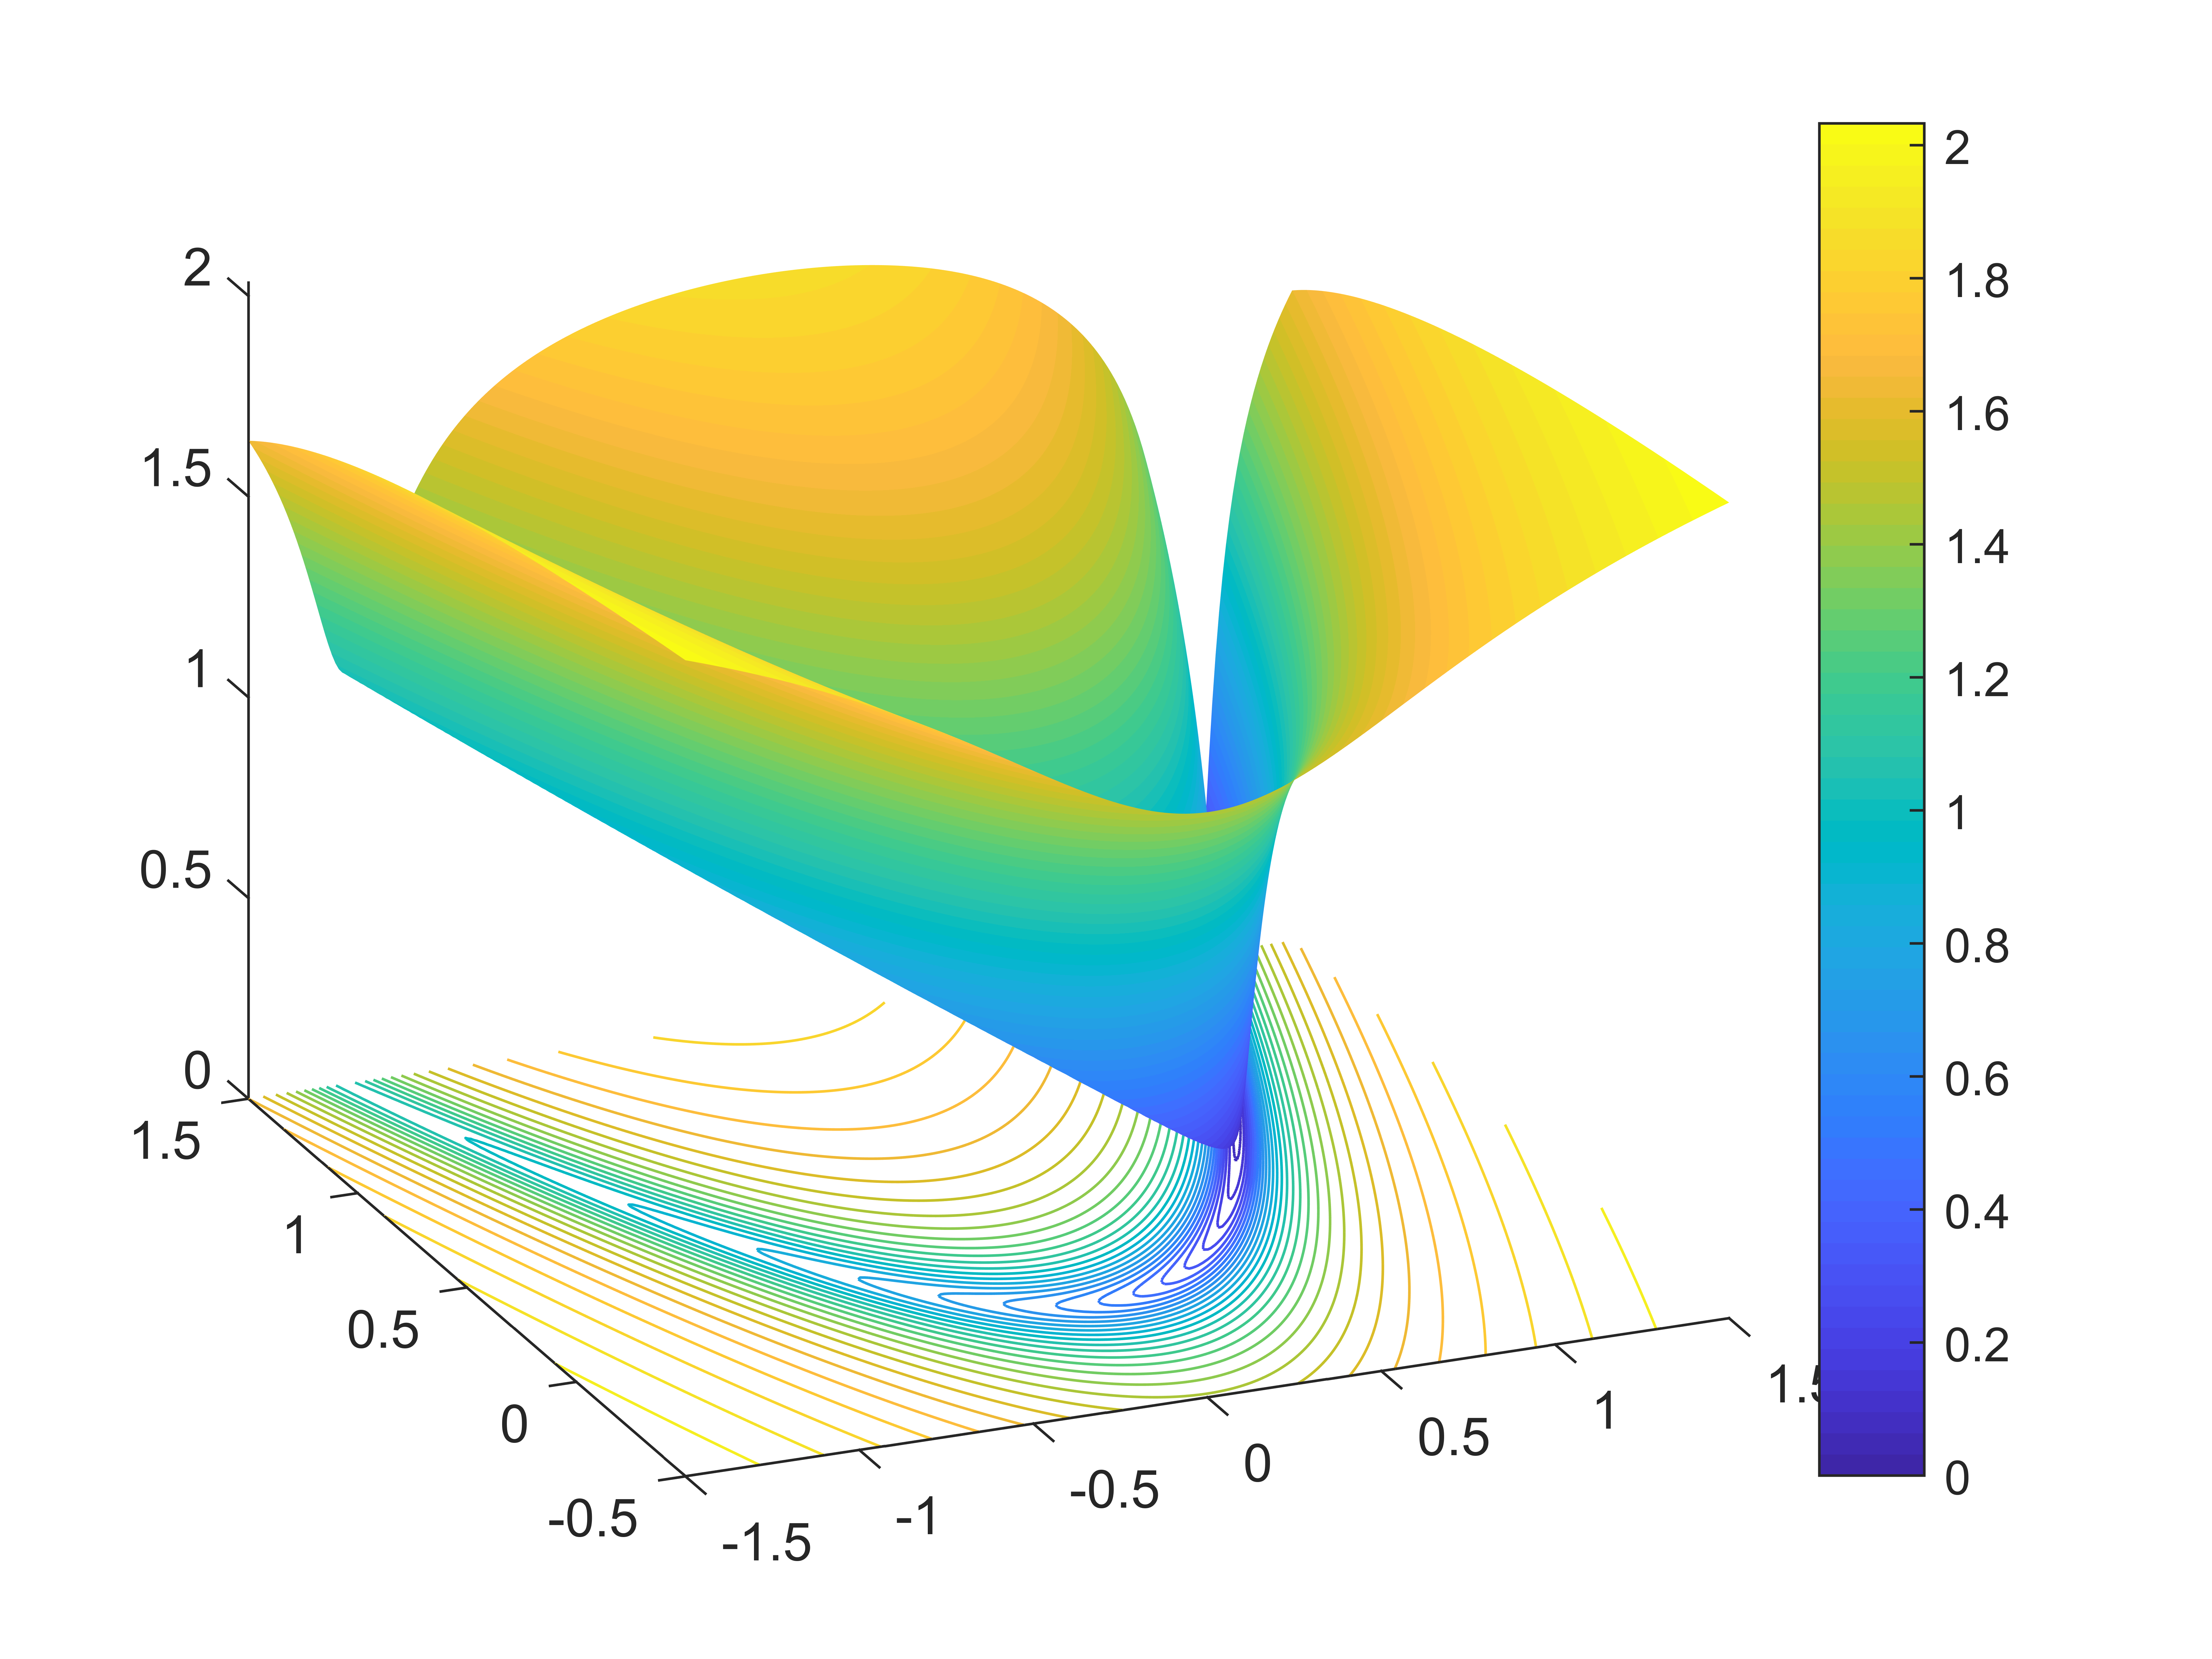
\includegraphics[width=11cm]{fig/4_02.png}
\end{figure}

\subsection{算法伪代码}
Armijo线搜索法参看上节的(\textbf{Algorithm} \ref{Amj})

带线搜索的Newton法算法参看上节的(\textbf{Algorithm} \ref{NewtonAmj})

\begin{algorithm}[h]  
\caption{Steepest-denscent-Armijo method for problem(5.9)}  
\begin{algorithmic}[1]  
\STATE Given $\bm{x}^{(0)}$ and $G$
\STATE Set $\bm{p}^{(0)}=-\bm{g}^{(0)},k=0$
\WHILE {$\|\bm{g}^{(k)}\|>\epsilon$}
\STATE Compute $\alpha_k$ by Line Search(\textbf{Algorithm} \ref{Amj})
\STATE Set $\bm{x}^{(k+1)}=\bm{x}^{(k)}+\alpha_k\bm{p}^{(k)}$
\STATE Set $\bm{g}^{(k+1)}=g(\bm{x}^{(k+1)})$
\STATE Set $\bm{p}^{(k)}=-\bm{g}^{(k)}$
\STATE Set $k=k+1$
\ENDWHILE
\end{algorithmic}  
\end{algorithm}



\subsection{计算结果展示}

本题中Armijo线搜索的参数为$\gamma=0.5,\rho=0.01$,并设置最大搜索步长为200.

然后分别以梯度下降法和牛顿法迭代,并画出等高线、运动轨迹、迭代值如下:

\begin{figure}[H]
\centering
\subfigure{
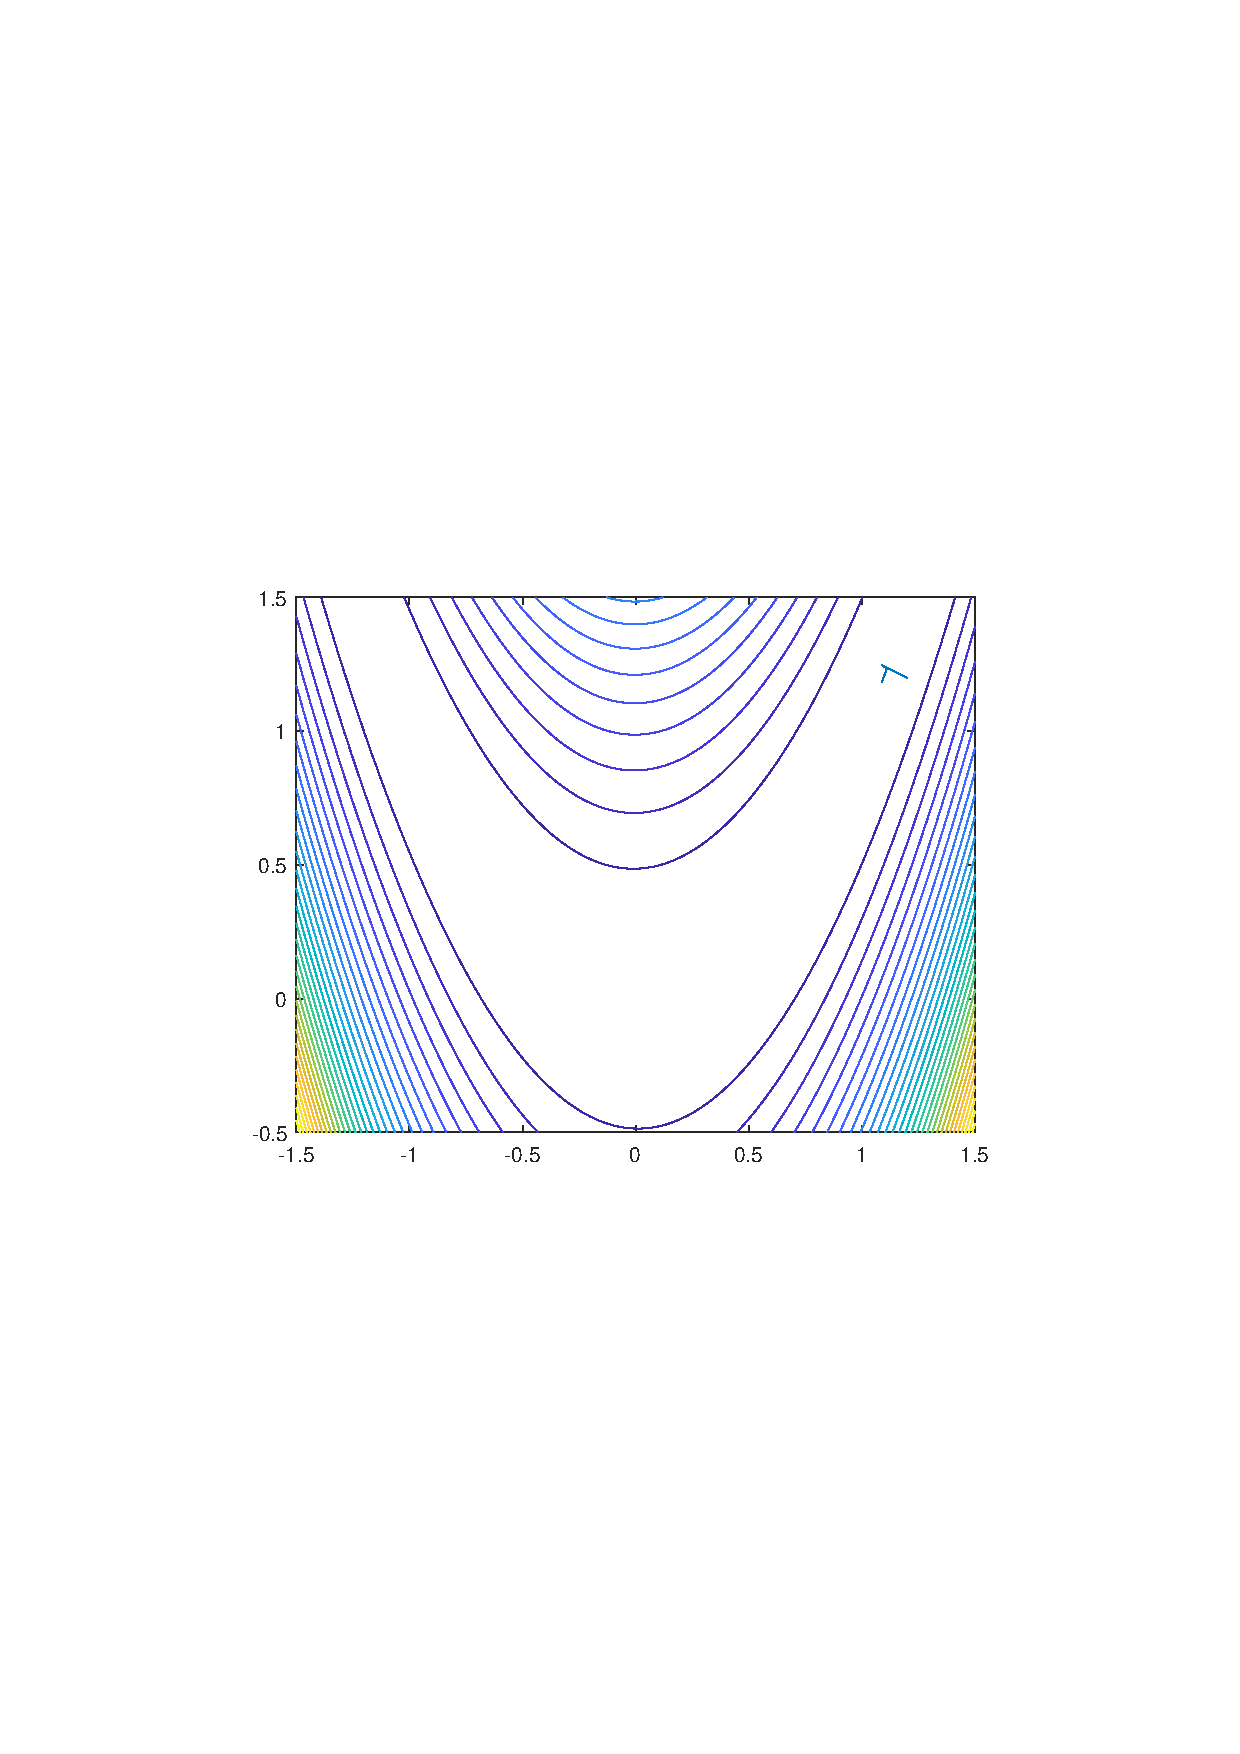
\includegraphics[width=5cm]{fig/4_11.pdf}}
\subfigure{
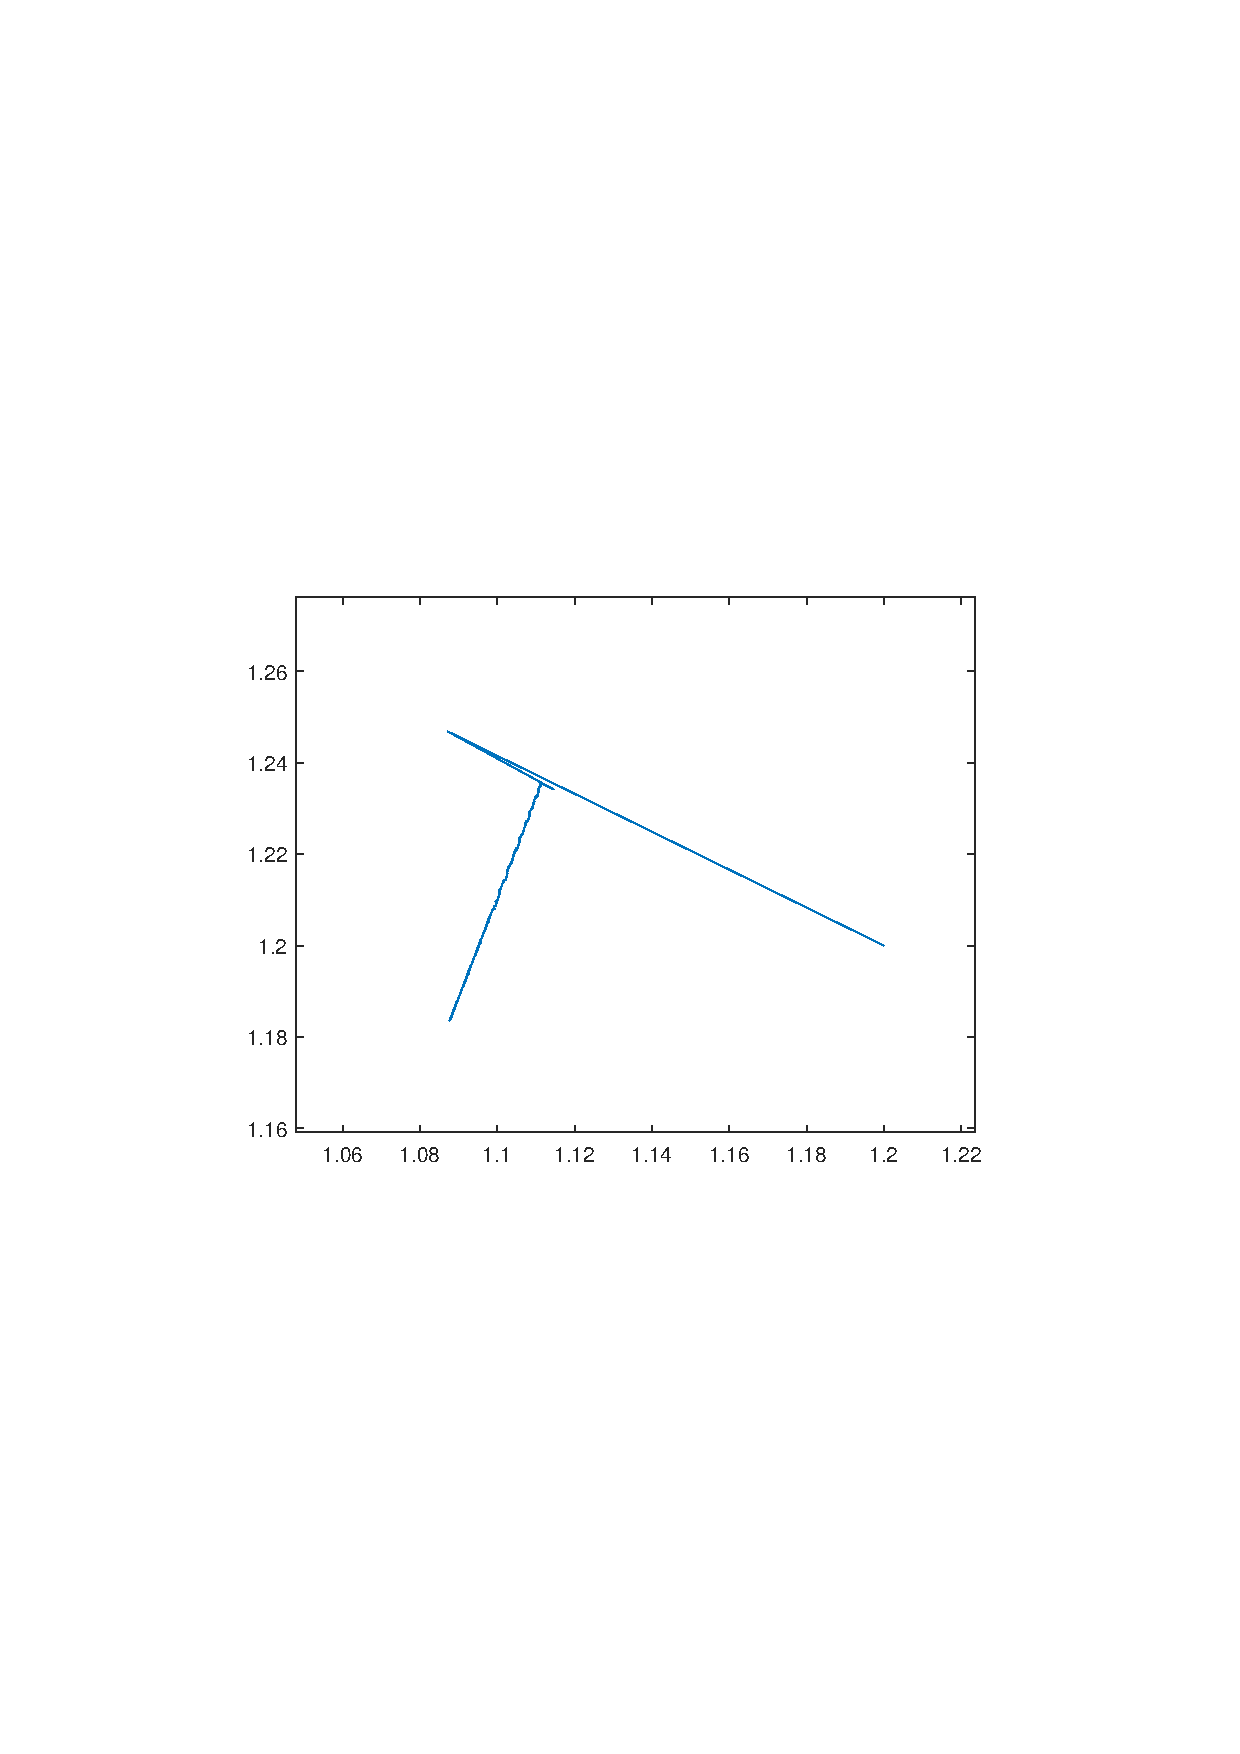
\includegraphics[width=5cm]{fig/4_12.pdf}}
\subfigure{
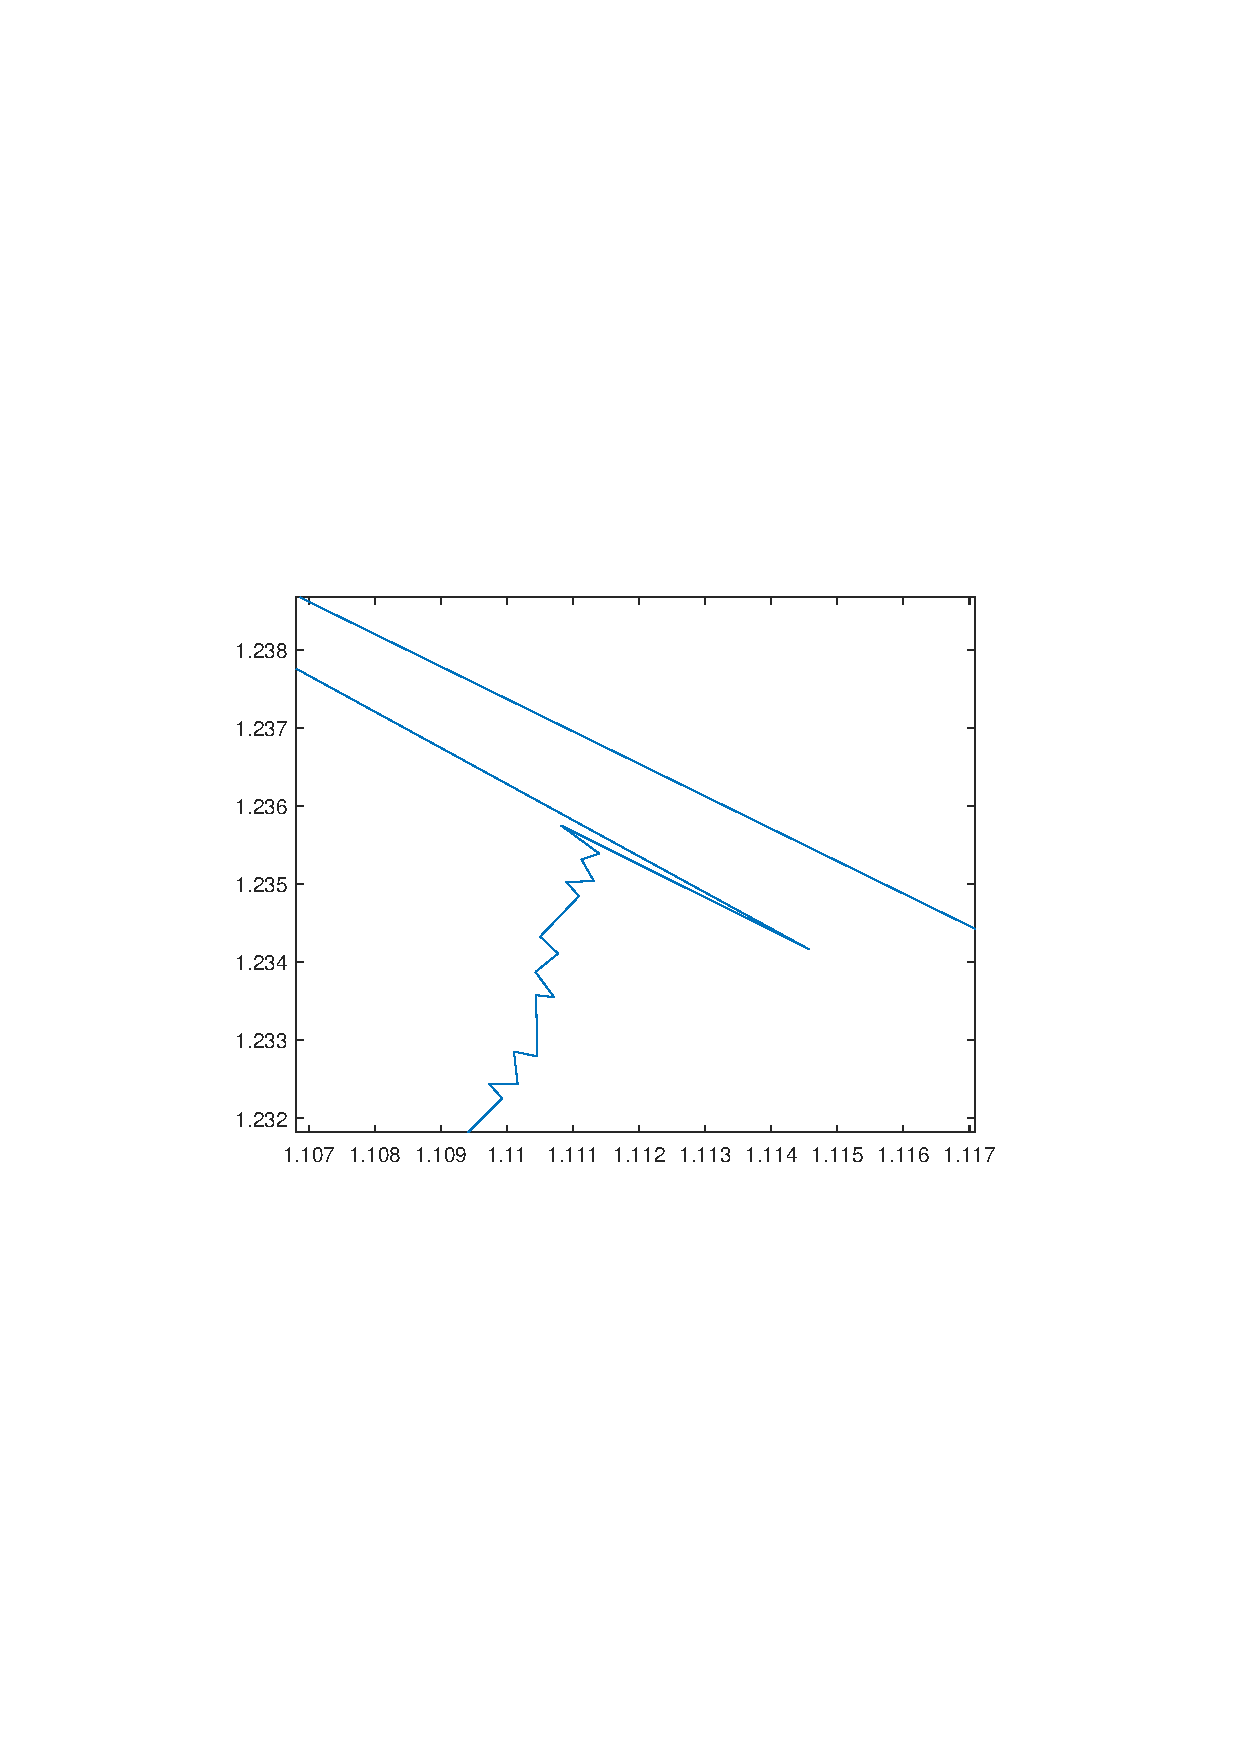
\includegraphics[width=5cm]{fig/4_13.pdf}}
\subfigure{
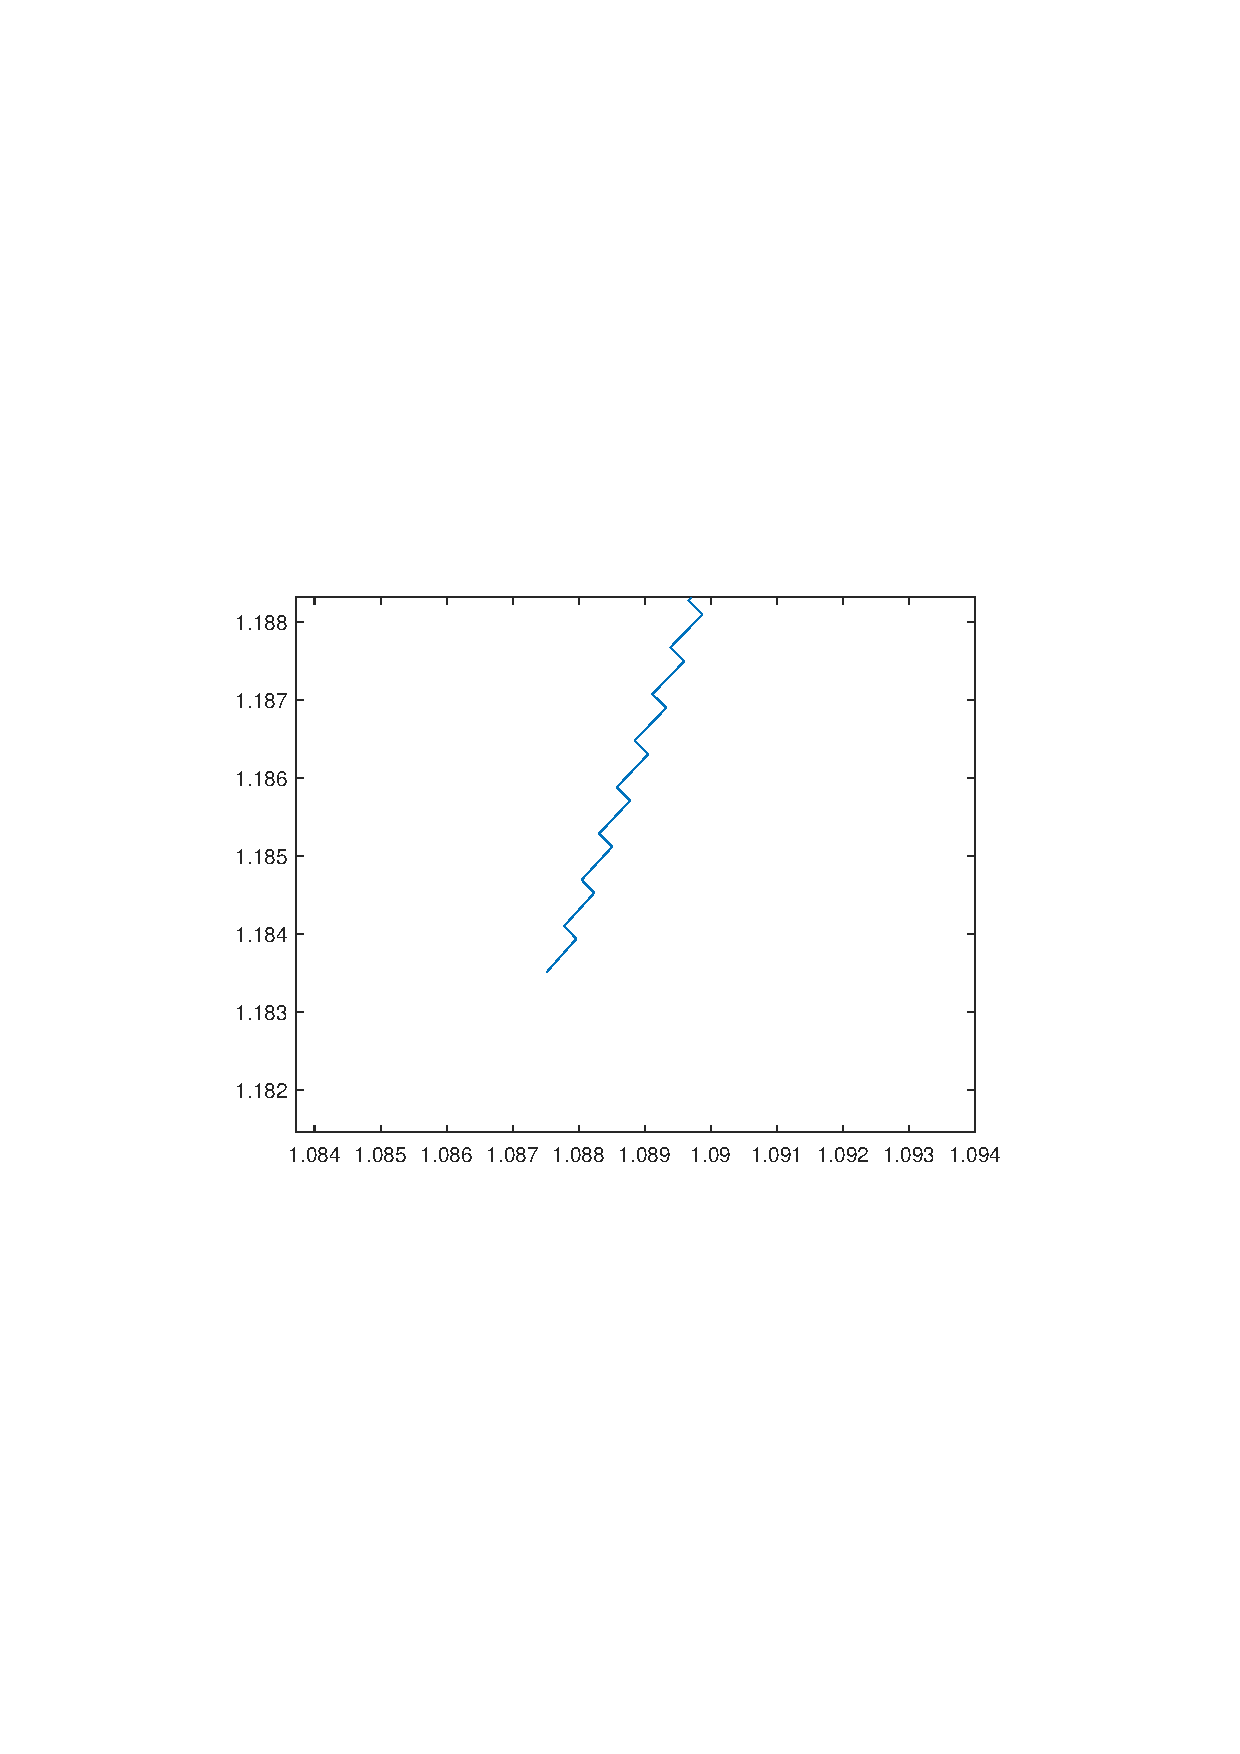
\includegraphics[width=5cm]{fig/4_14.pdf}}
\caption{Steepest-denscent in (1.2,1.2)}
\label{Fig.lable}
\end{figure}
\begin{lstlisting}
%Result for Steepest-denscent in (1.2,1.2)
Step[1]:  x=[ 1.200000 1.200000 ] optim_fx=5.800000
Step[2]:  x=[ 1.087109 1.246875 ] optim_fx=0.430975
Step[3]:  x=[ 1.114571 1.234166 ] optim_fx=0.019689
...
...
...
Step[198]:  x=[ 1.083582 1.174725 ] optim_fx=0.007019
Step[199]:  x=[ 1.083742 1.174500 ] optim_fx=0.007013
Step[200]:  x=[ 1.083580 1.174500 ] optim_fx=0.006998
%最速下降法,共迭代 200 步
%最优解:
x=[ 1.083580e+00 1.174500e+00 ] optim_fx=0.006998
\end{lstlisting}

\begin{figure}[H]
\centering
\subfigure{
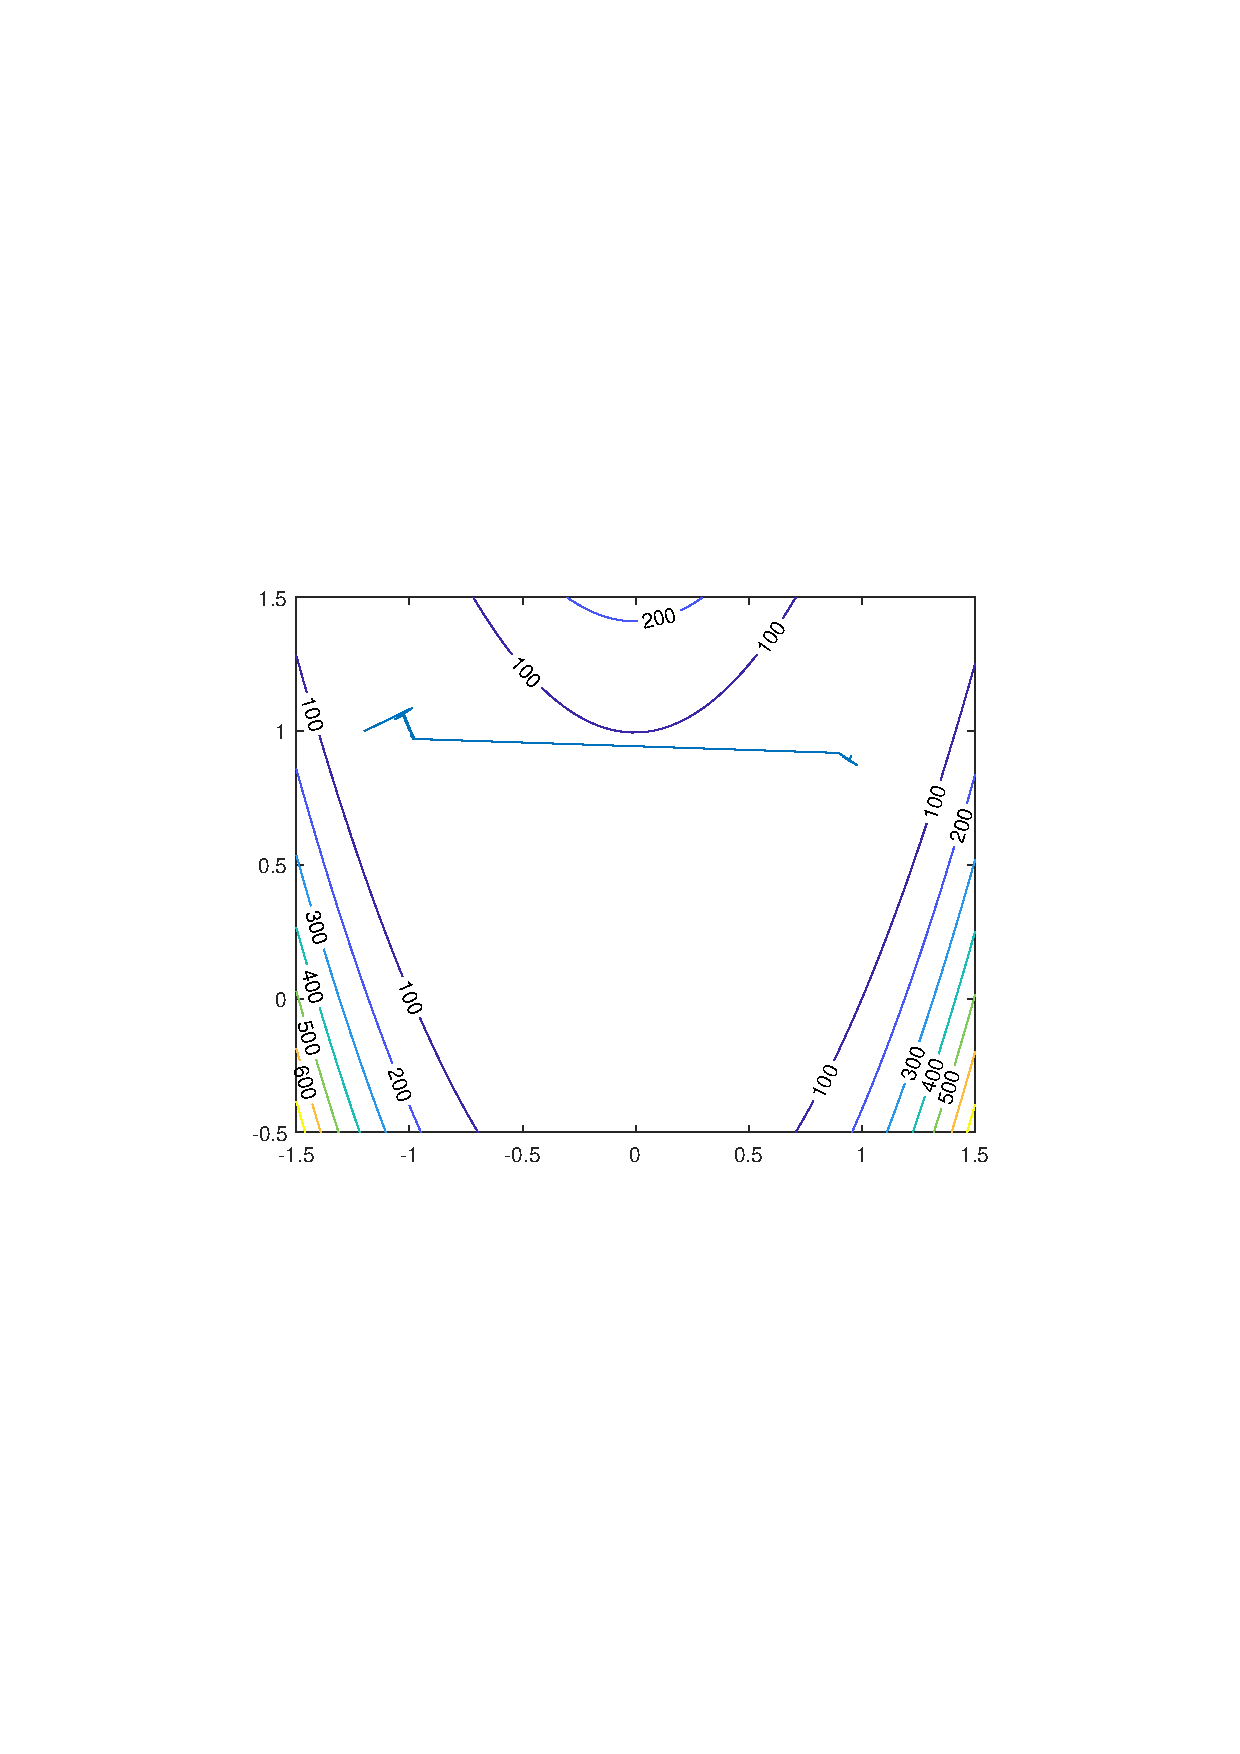
\includegraphics[width=5cm]{fig/4_21.pdf}}
\subfigure{
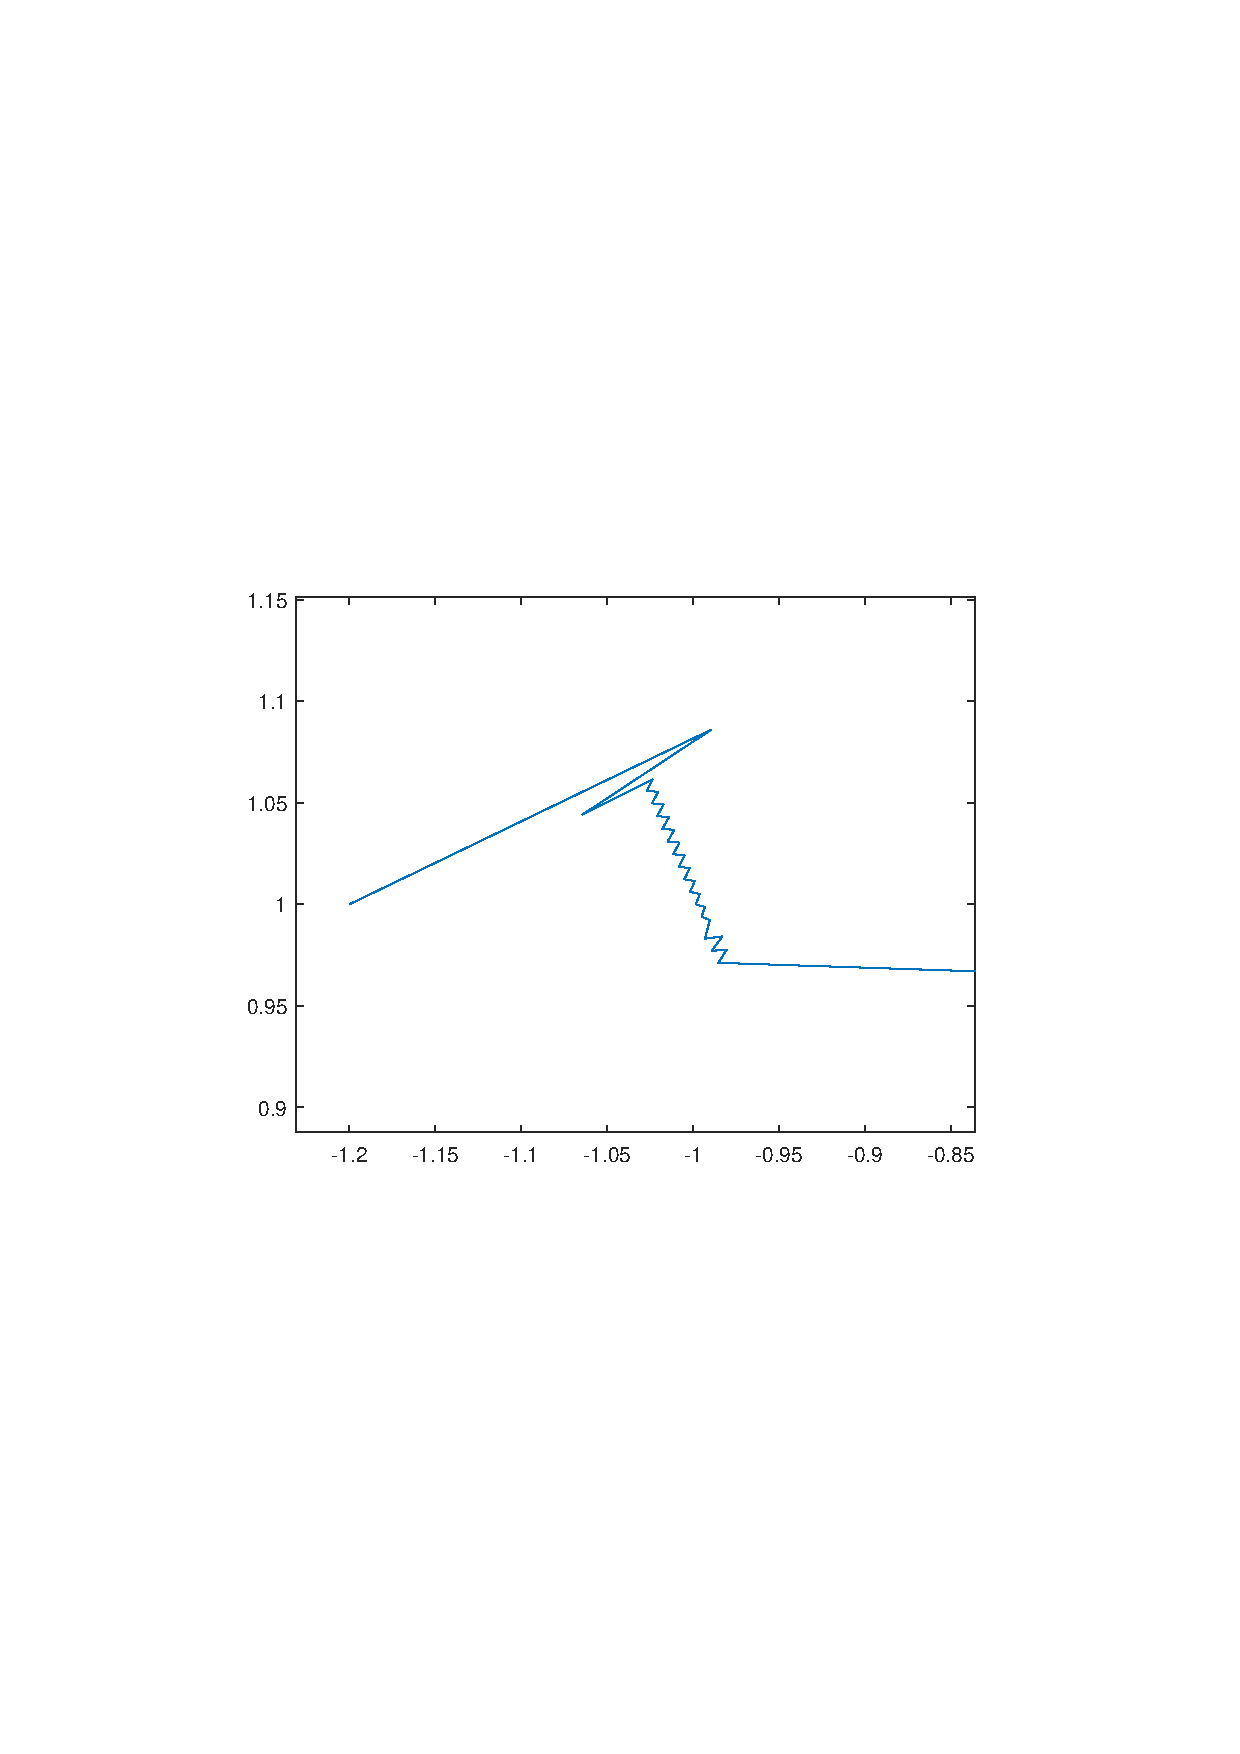
\includegraphics[width=5cm]{fig/4_22.pdf}}
\subfigure{
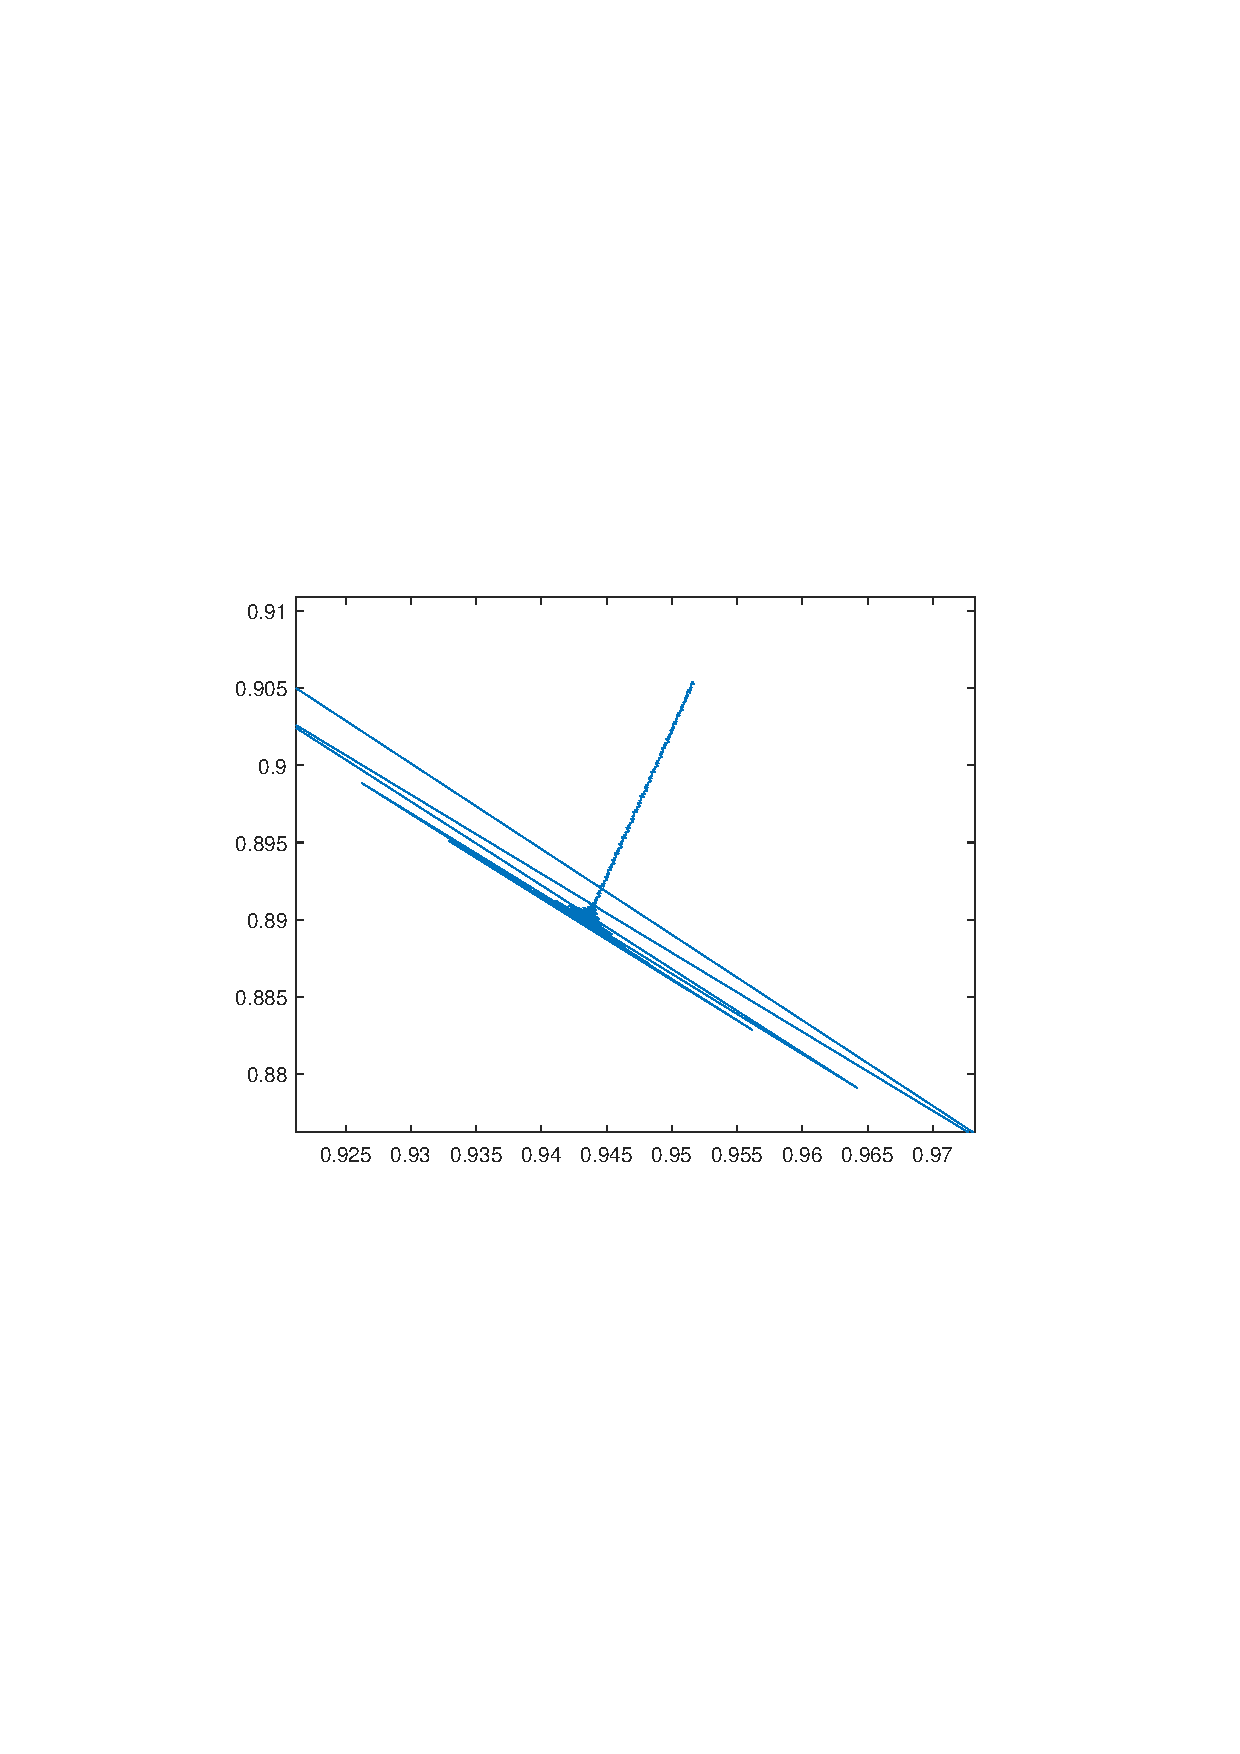
\includegraphics[width=5cm]{fig/4_23.pdf}}
\subfigure{
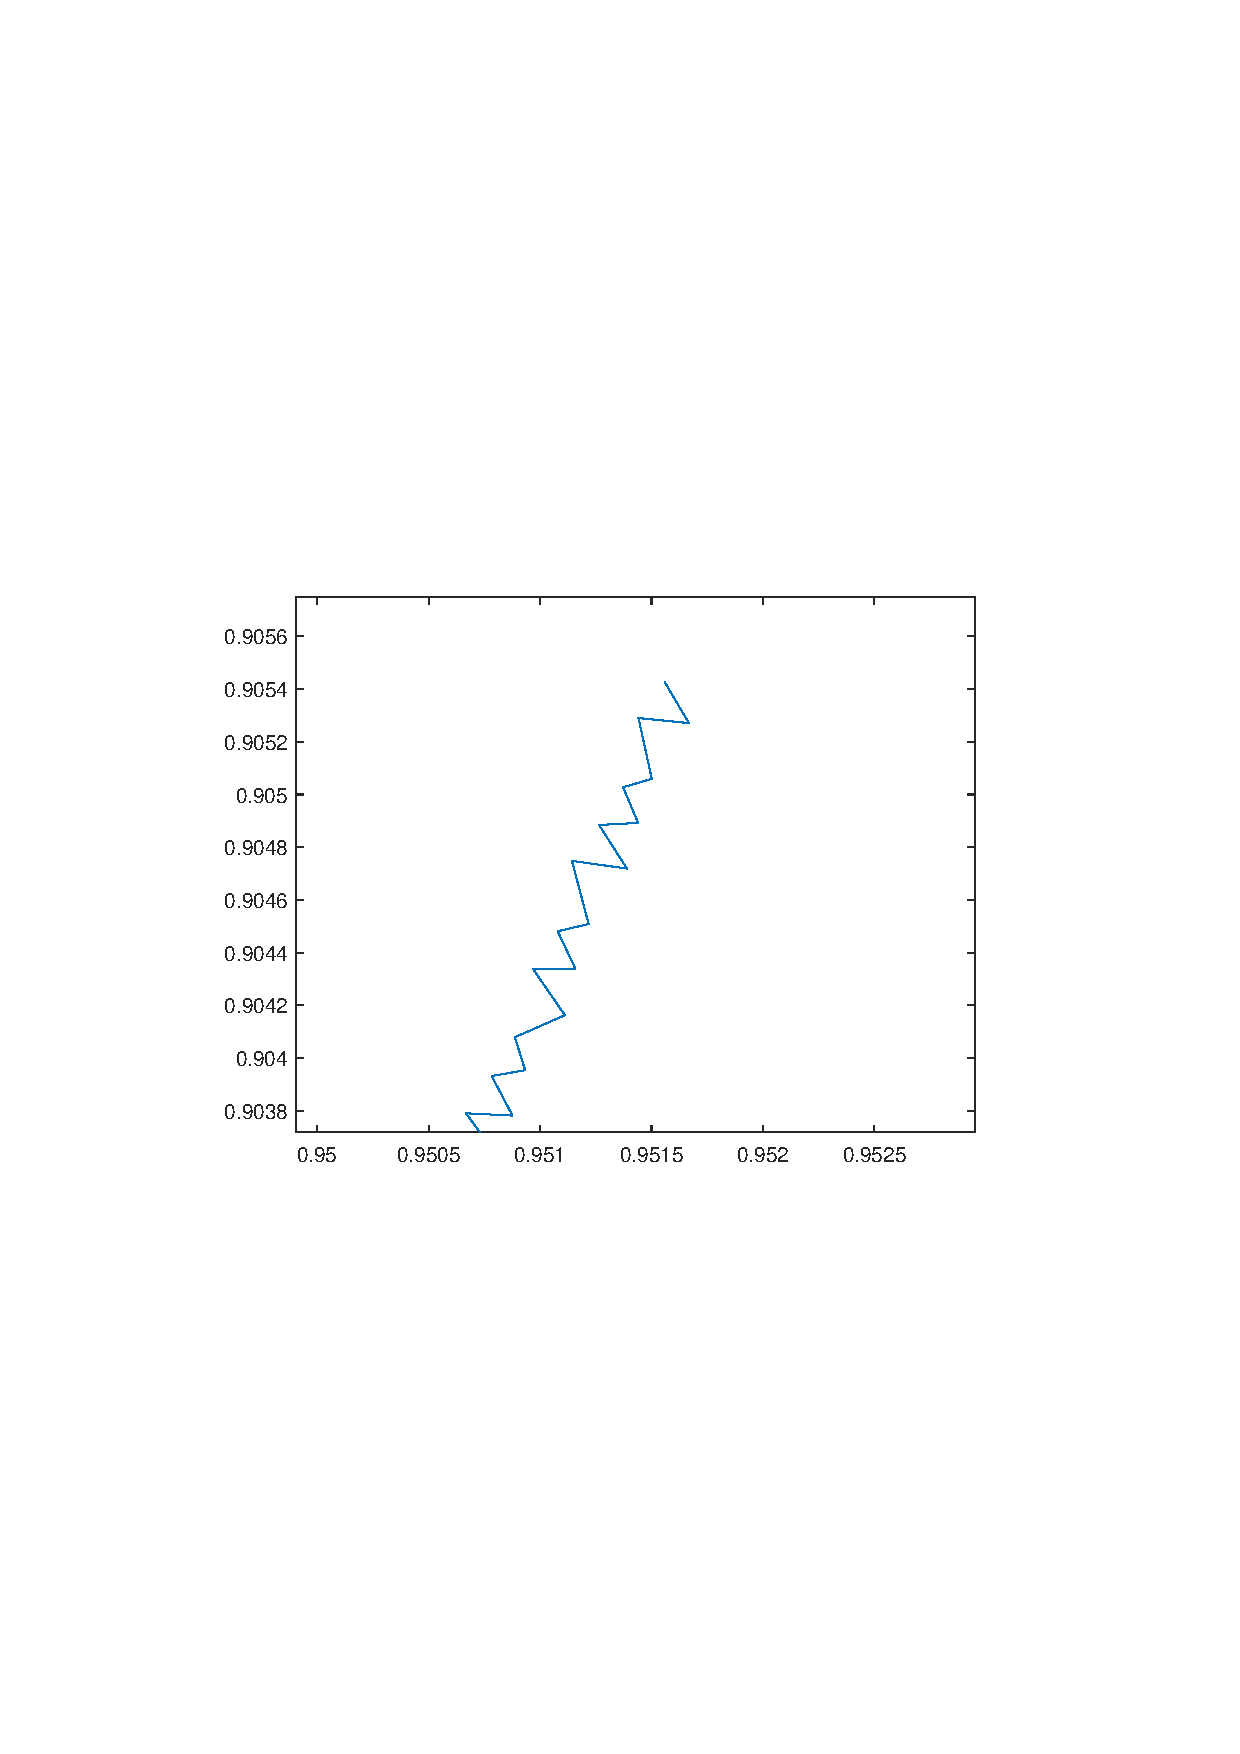
\includegraphics[width=5cm]{fig/4_24.pdf}}
\caption{Steepest-denscent in (-1.2,1)}
\label{Fig.lable}
\end{figure}

\begin{lstlisting}
%Result for Steepest-denscent in (-1.2,1)
Step[1]:  x=[ -1.200000 1.000000 ] optim_fx=24.200000
Step[2]:  x=[ -0.989453 1.085938 ] optim_fx=5.101113
Step[3]:  x=[ -1.026893 1.065055 ] optim_fx=4.119416
Step[4]:  x=[ -1.027979 1.056815 ] optim_fx=4.112700
Step[5]:  x=[ 0.984742 1.049394 ] optim_fx=0.635080
Step[6]:  x=[ 1.015421 1.033832 ] optim_fx=0.000995
...
...
...
Step[195]:  x=[ 1.005171 1.010402 ] optim_fx=0.000027
Step[196]:  x=[ 1.005177 1.010389 ] optim_fx=0.000027
Step[197]:  x=[ 1.005163 1.010386 ] optim_fx=0.000027
Step[198]:  x=[ 1.005169 1.010373 ] optim_fx=0.000027
Step[199]:  x=[ 1.005155 1.010370 ] optim_fx=0.000027
Step[200]:  x=[ 1.005161 1.010357 ] optim_fx=0.000027
%最速下降法,共迭代 200 步
%最优解:
x=[ 1.005161e+00 1.010357e+00 ] optim_fx=0.000027
\end{lstlisting}

\begin{figure}[H]
\centering
\subfigure{
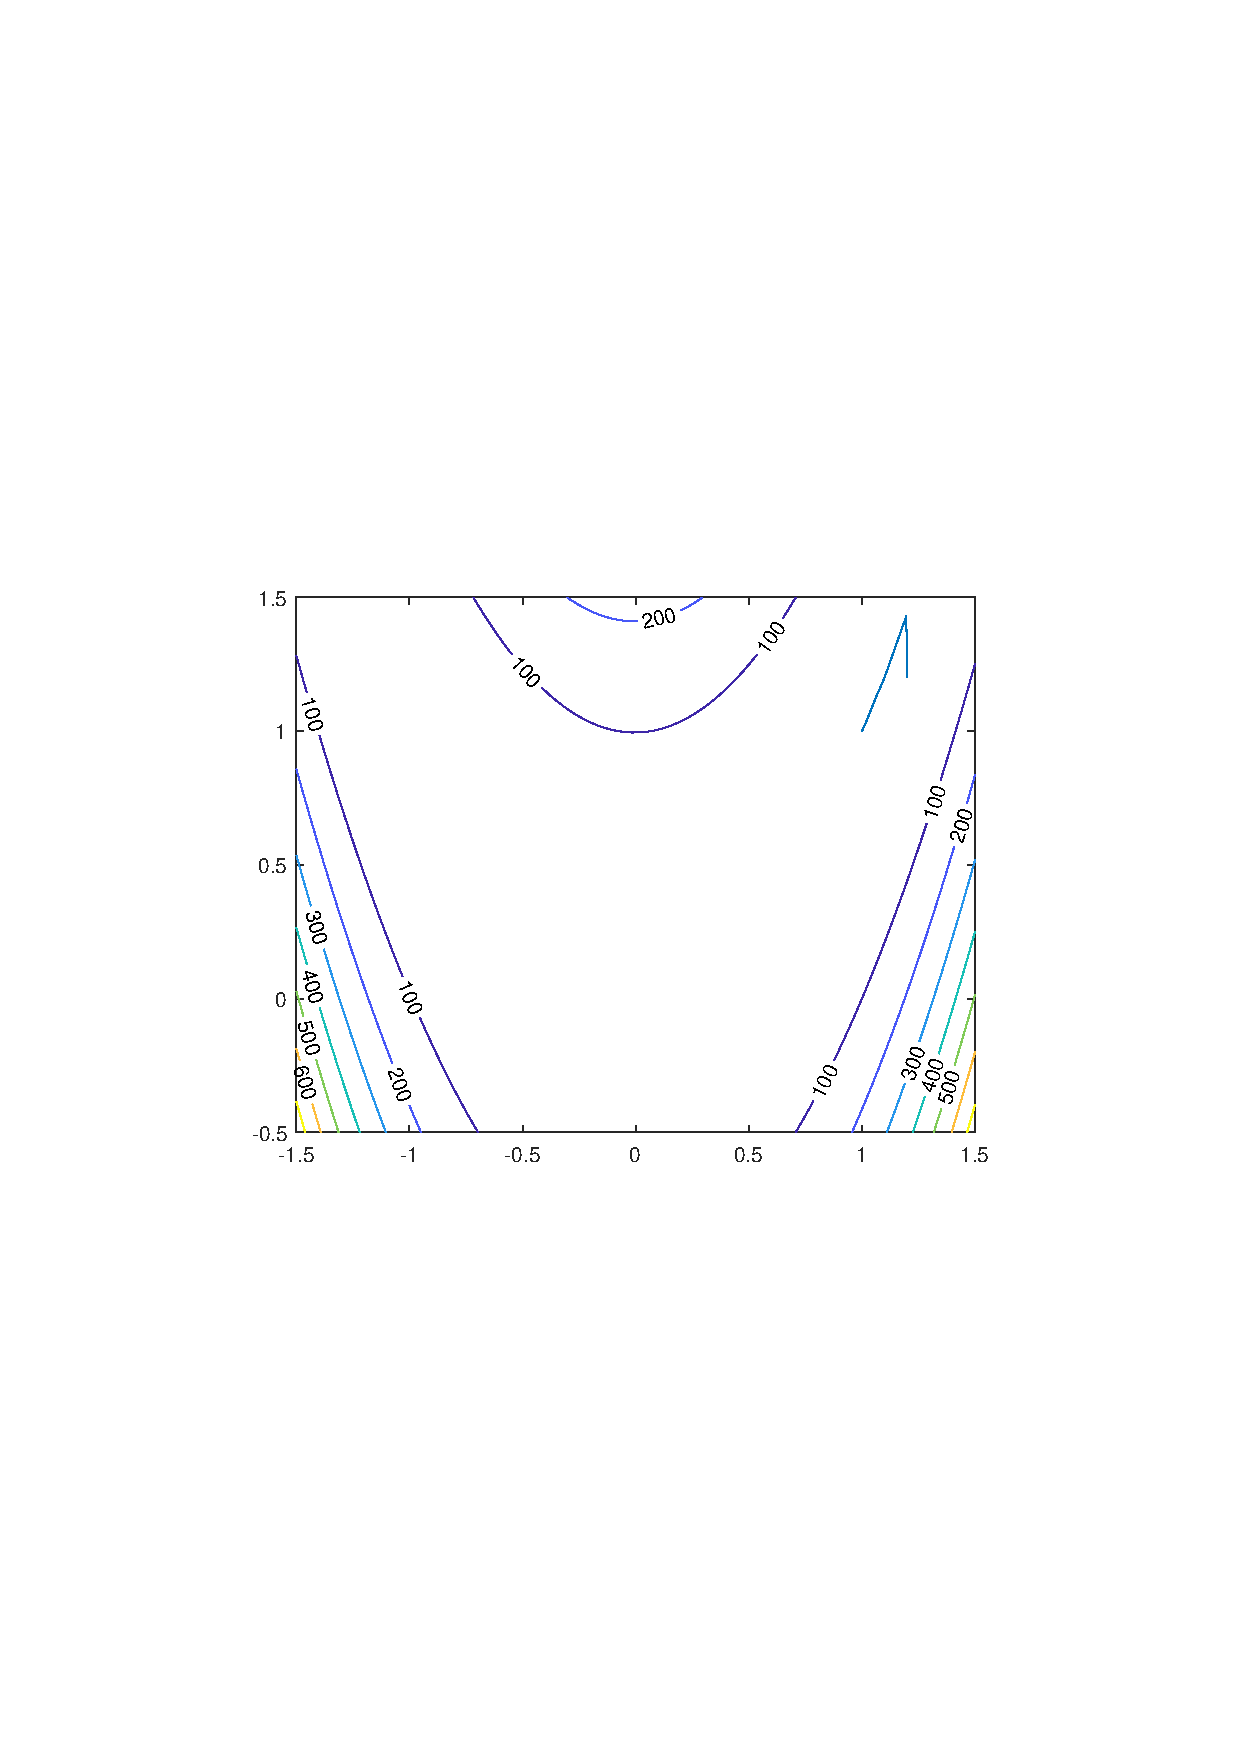
\includegraphics[width=5cm]{fig/4_31.pdf}}
\subfigure{
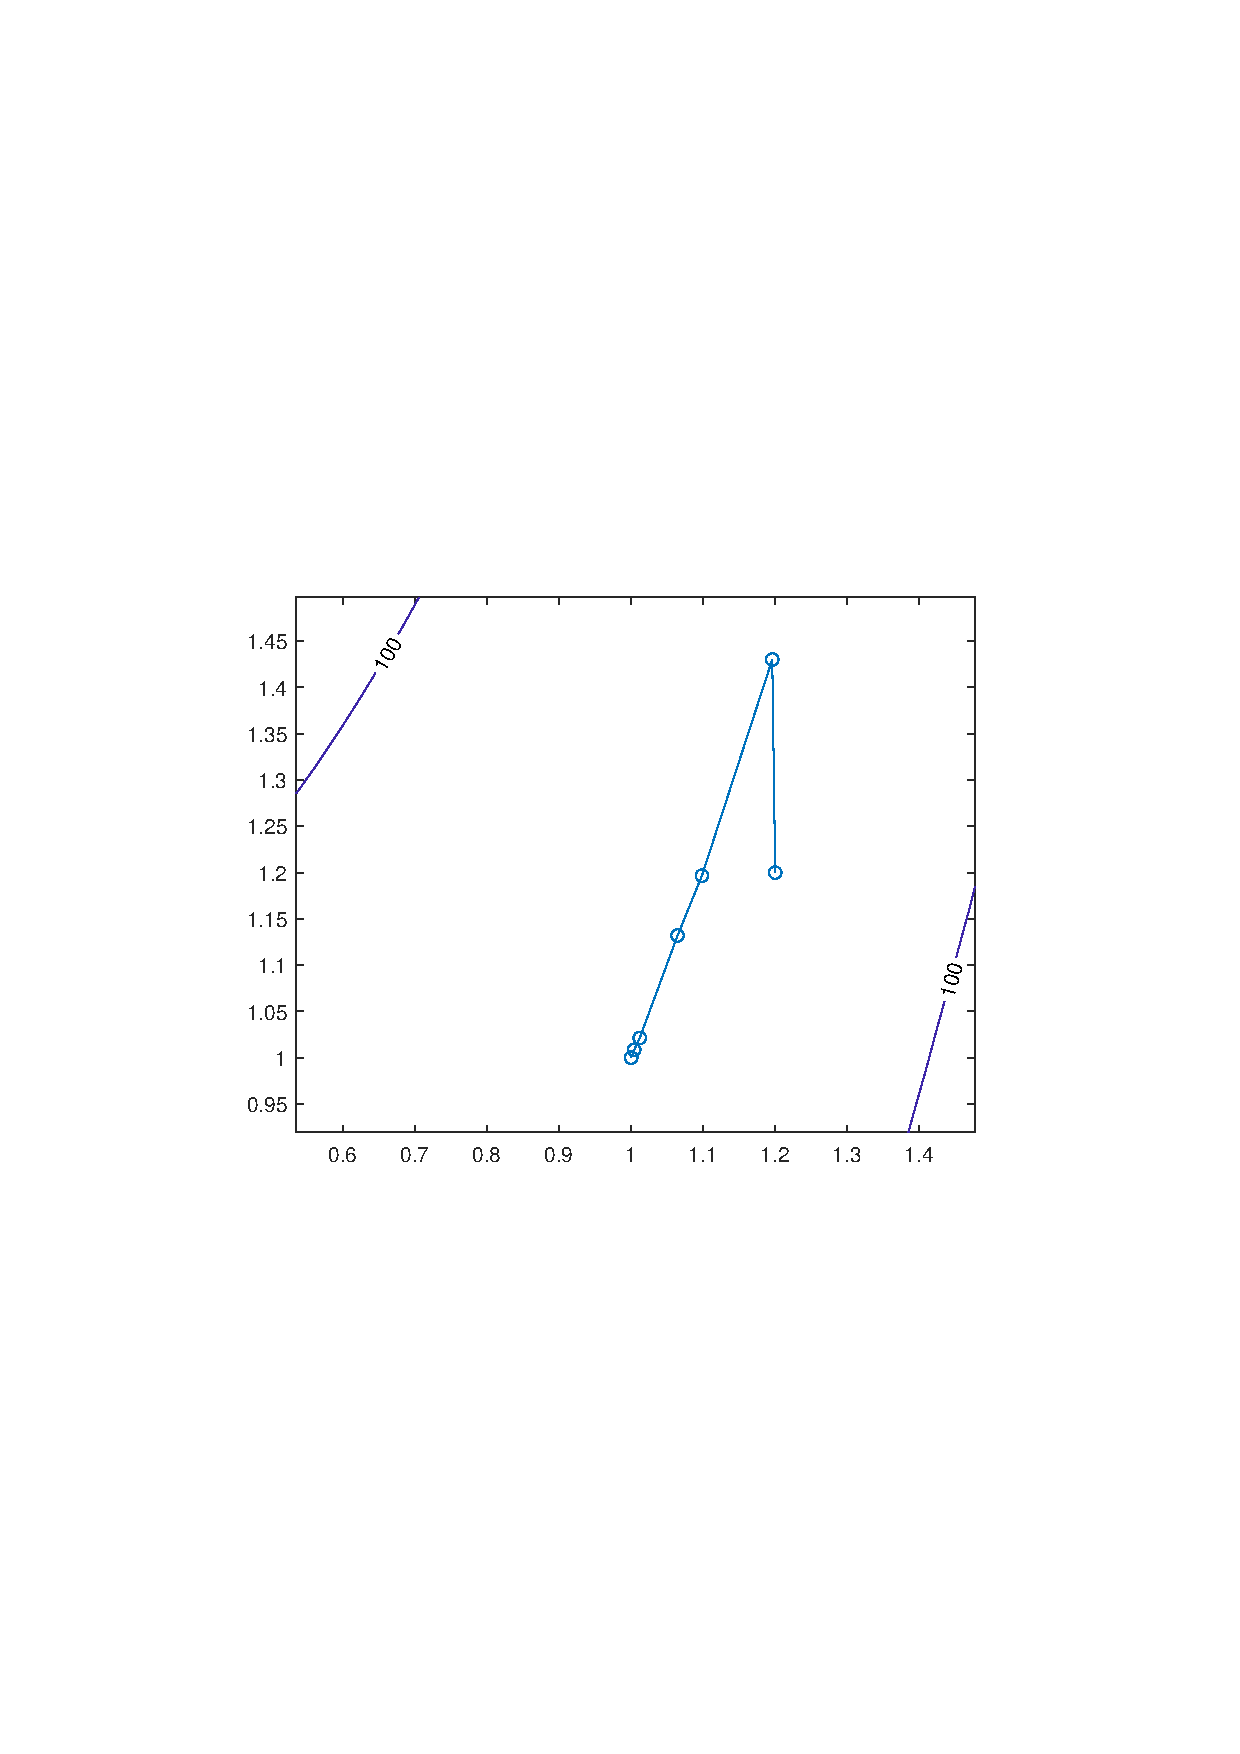
\includegraphics[width=5cm]{fig/4_32.pdf}}
\subfigure{
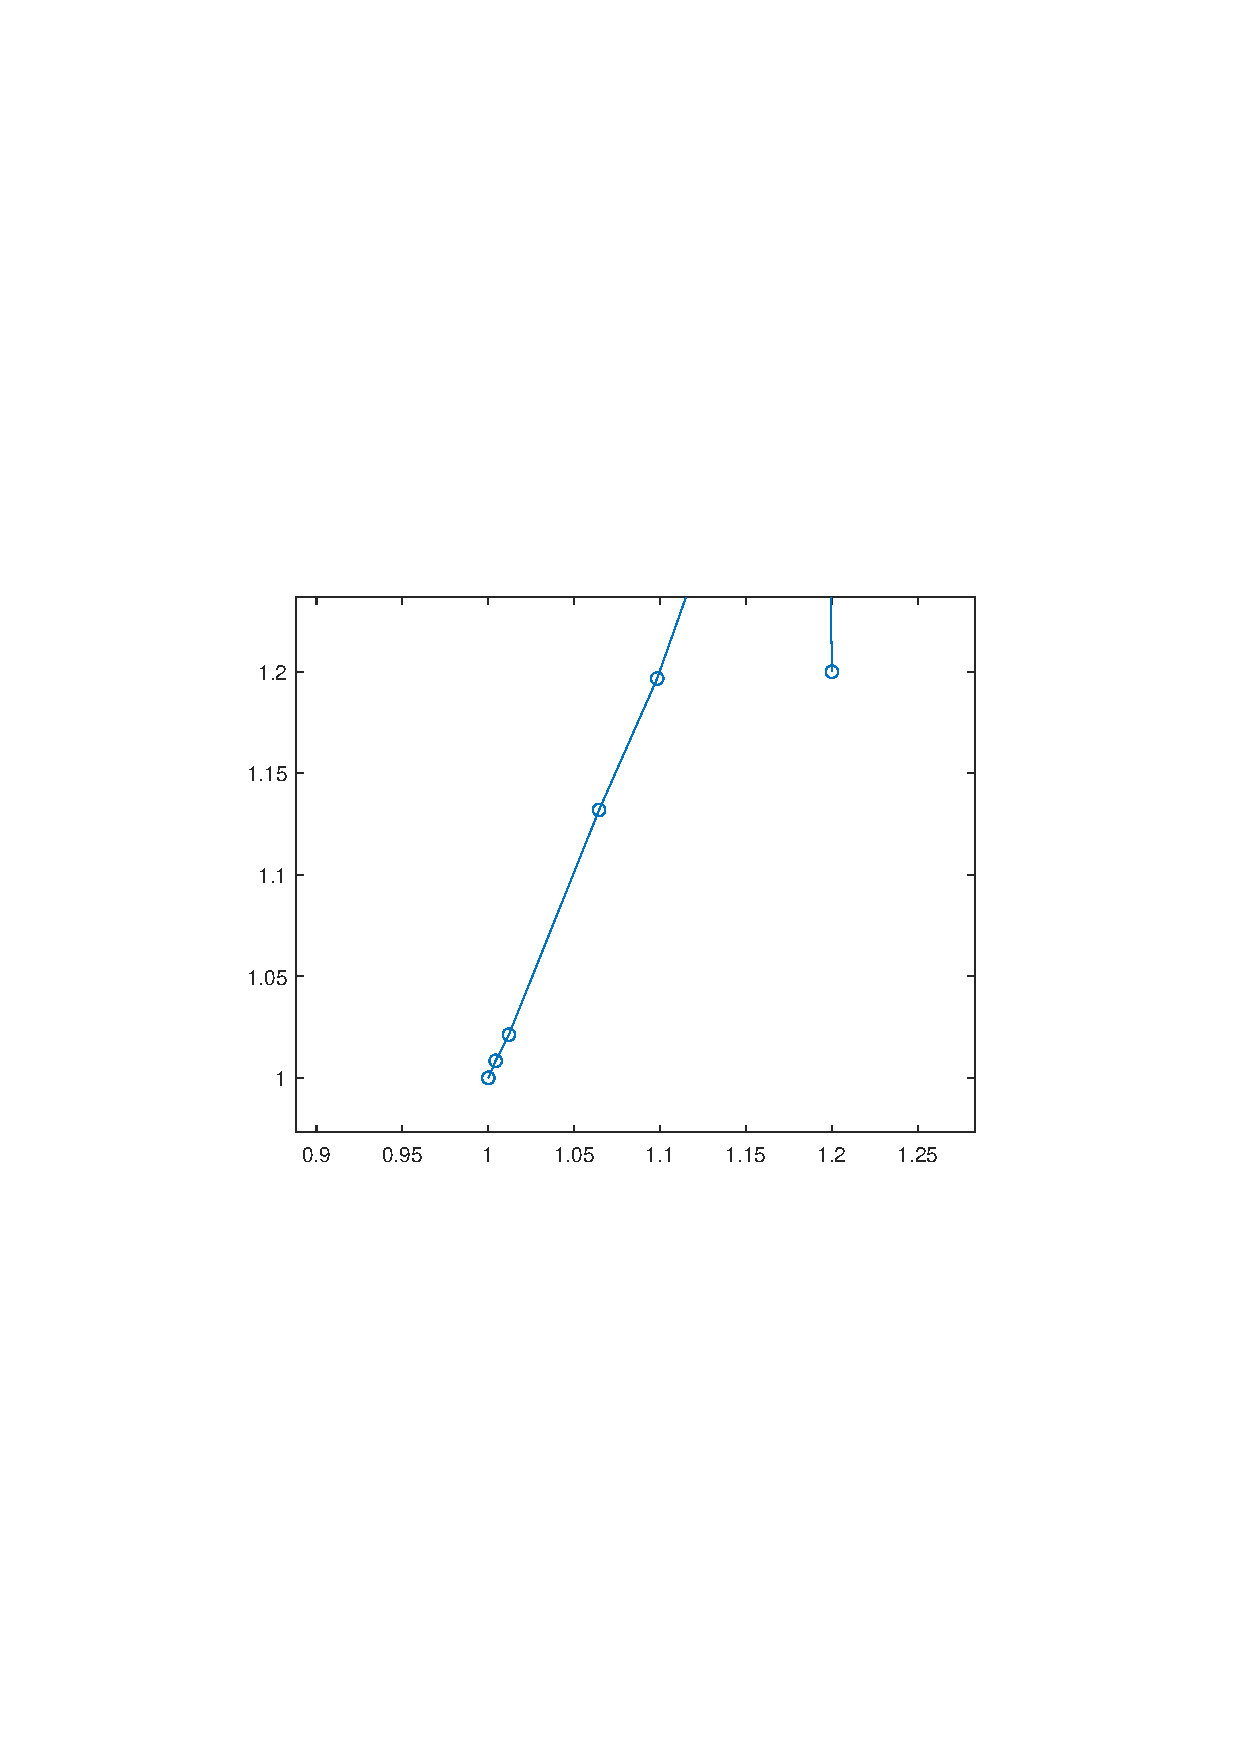
\includegraphics[width=5cm]{fig/4_33.pdf}}
\subfigure{
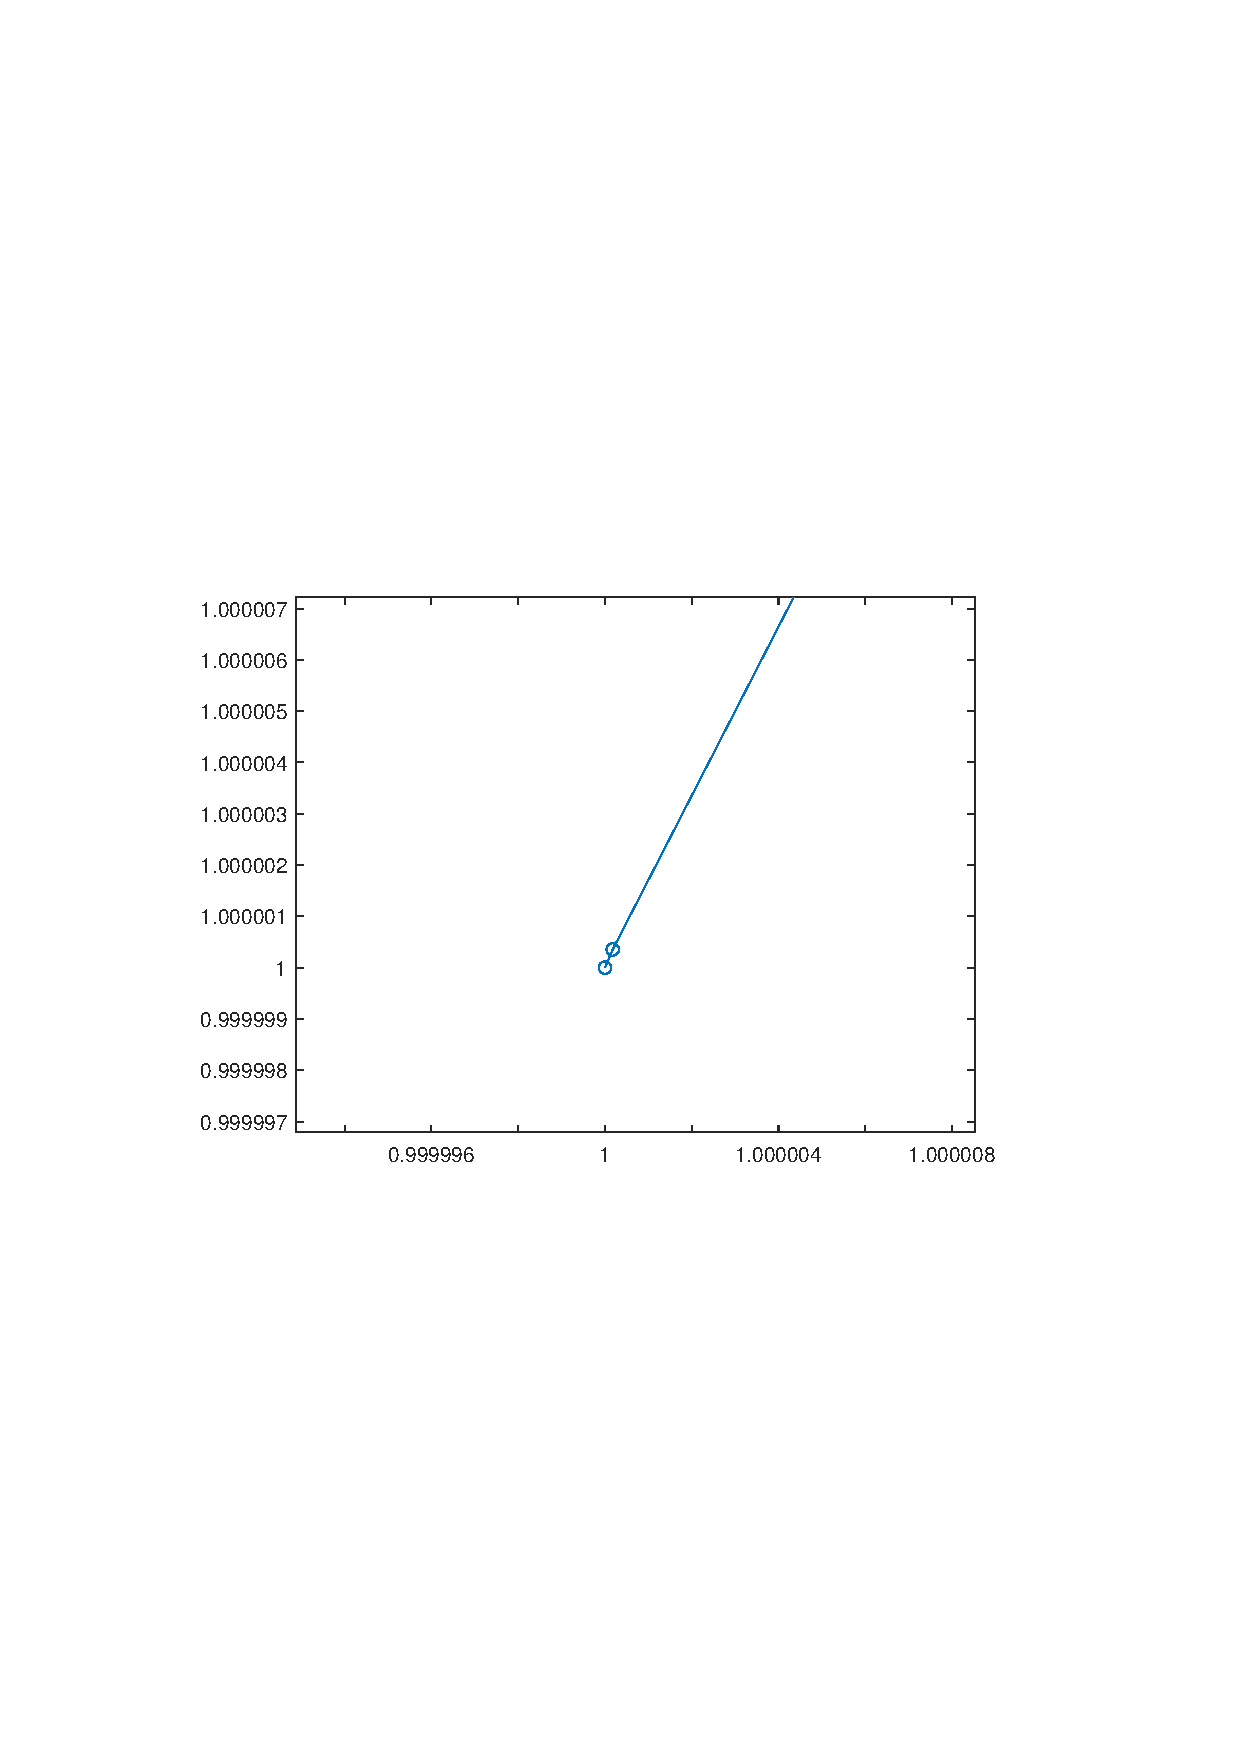
\includegraphics[width=5.3cm]{fig/4_34.pdf}}
\caption{Newton-Armijo in (1.2,1.2)}
\label{Fig.lable}
\end{figure}

\begin{lstlisting}
%Result for Newton-Armijo in (1.2,1.2)
Step[1]: x=[ 1.200000 1.200000 ] optim_fx=5.800000
Step[2]: x=[ 1.195918 1.430204 ] optim_fx=0.038384
Step[3]: x=[ 1.098284 1.196688 ] optim_fx=0.018762
Step[4]: x=[ 1.064488 1.131993 ] optim_fx=0.004289
Step[5]: x=[ 1.011992 1.021372 ] optim_fx=0.000903
Step[6]: x=[ 1.004261 1.008481 ] optim_fx=0.000019
Step[7]: x=[ 1.000050 1.000083 ] optim_fx=0.000000
Step[8]: x=[ 1.000000 1.000000 ] optim_fx=0.000000
Step[9]: x=[ 1.000000 1.000000 ] optim_fx=0.000000
%牛顿 Armijo 回溯法,,共迭代 9 步
%最优解:
x=[ 1.000000e+00 1.000000e+00 ] optim_fx=0.000000
\end{lstlisting}

\begin{figure}[H]
\centering
\subfigure{
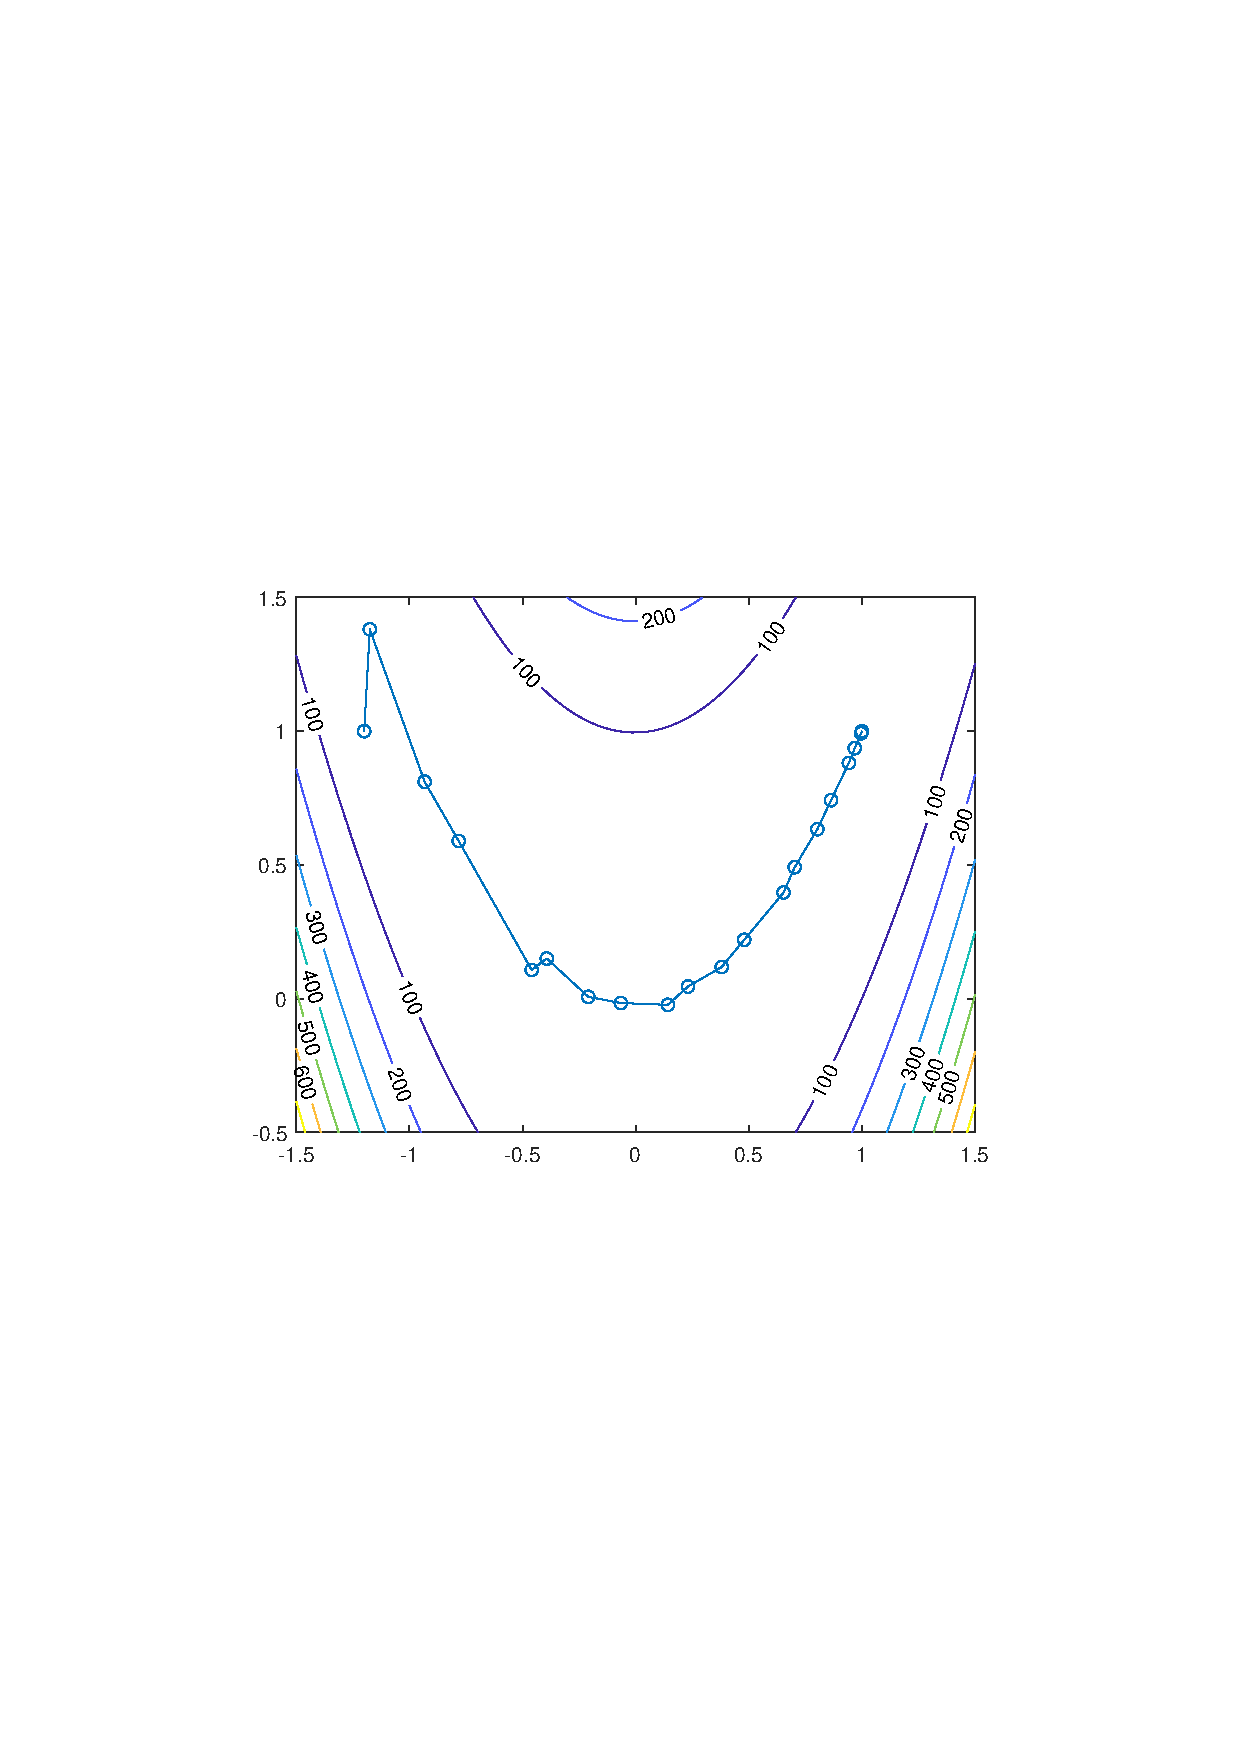
\includegraphics[width=5cm]{fig/4_41.pdf}}
\subfigure{
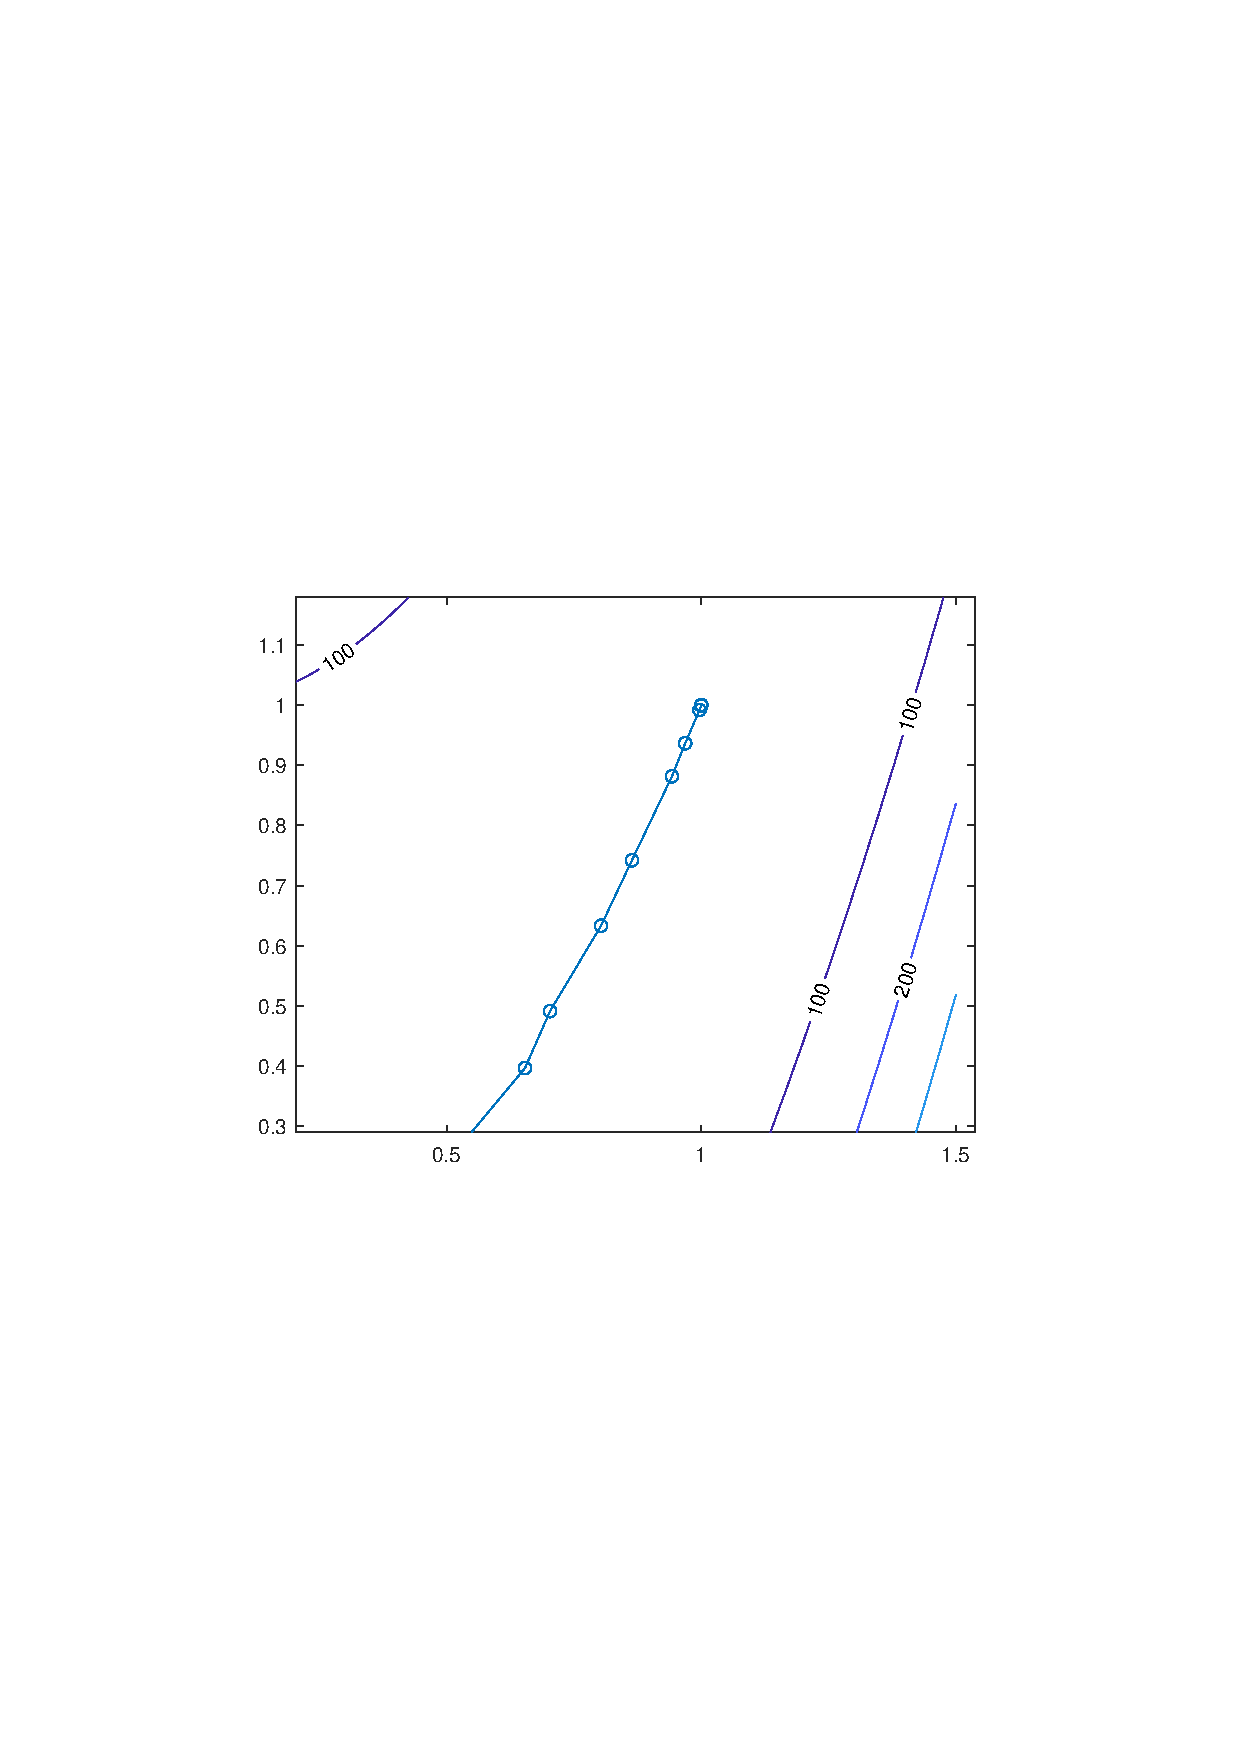
\includegraphics[width=5cm]{fig/4_42.pdf}}
\subfigure{
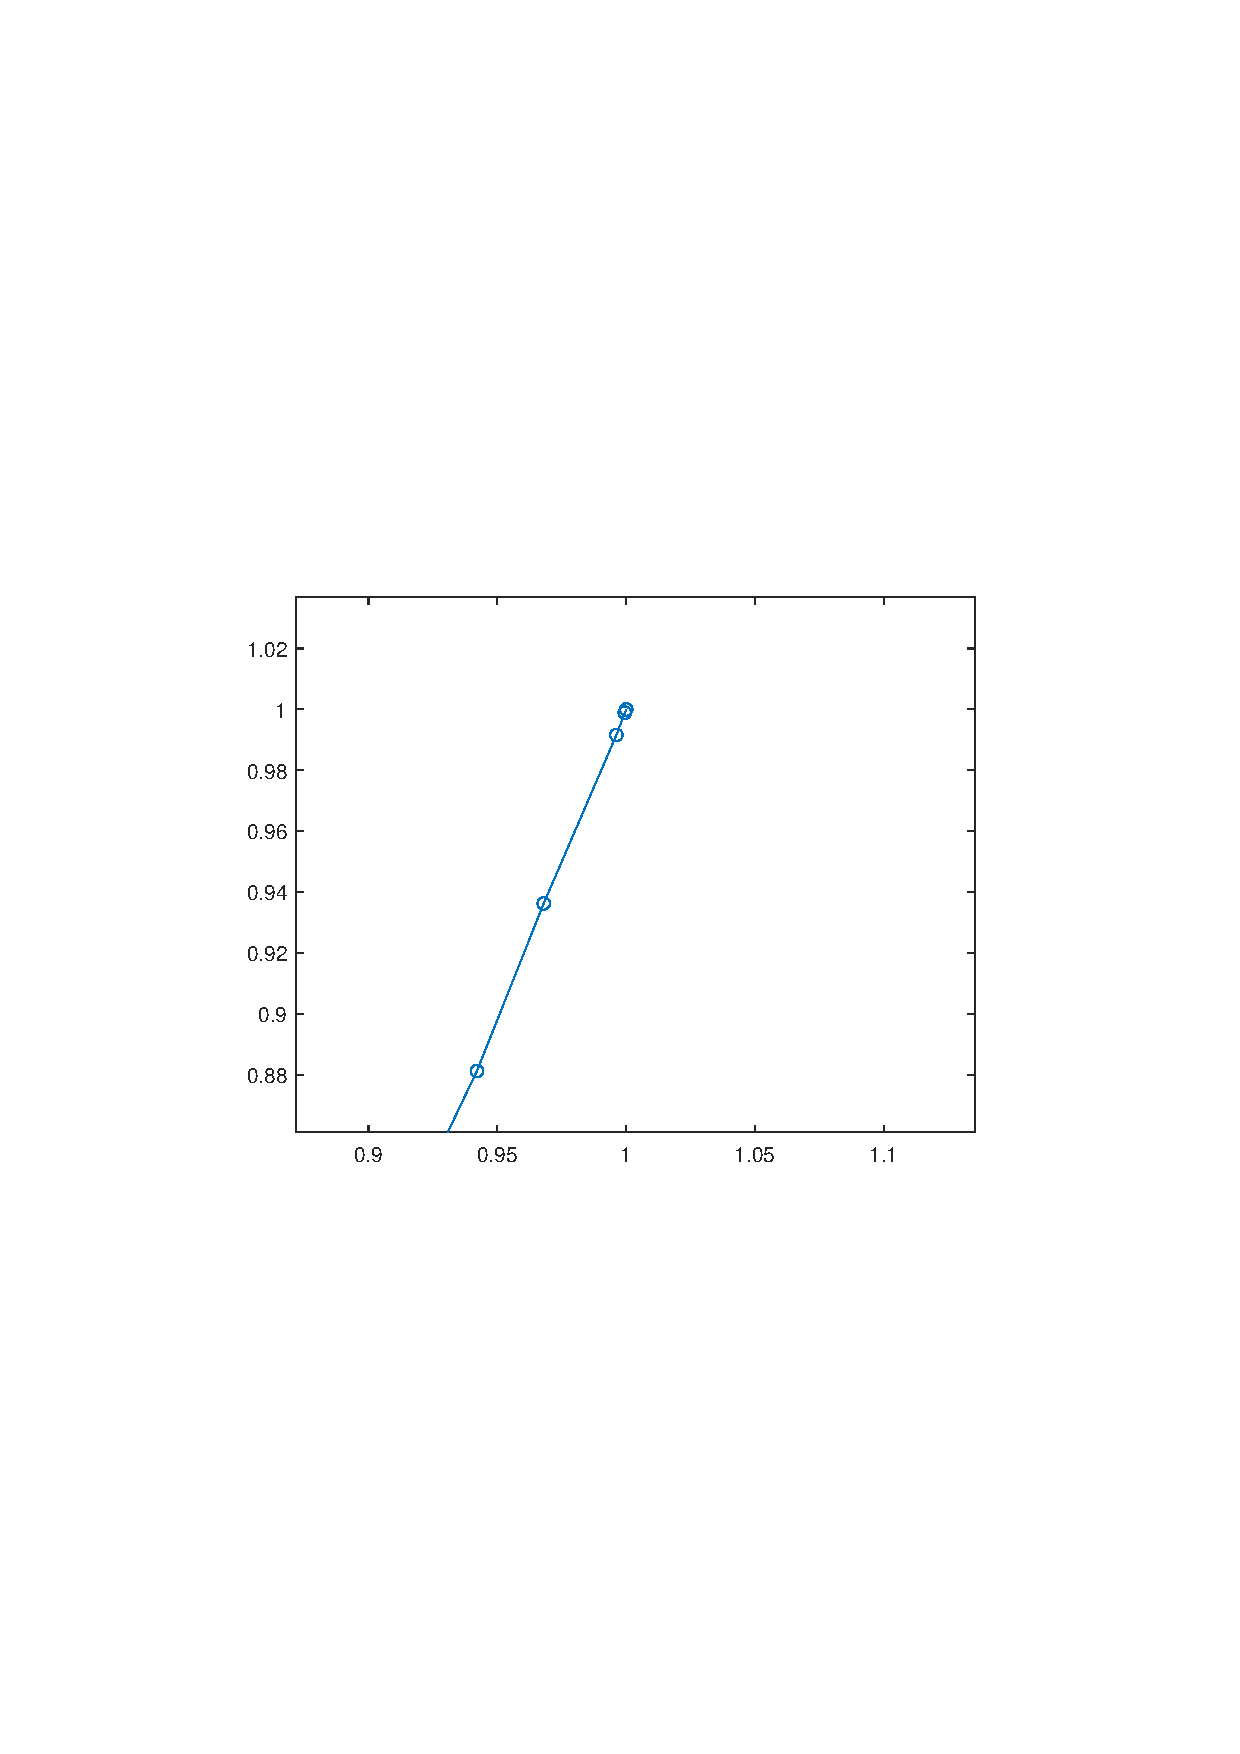
\includegraphics[width=5cm]{fig/4_43.pdf}}
\subfigure{
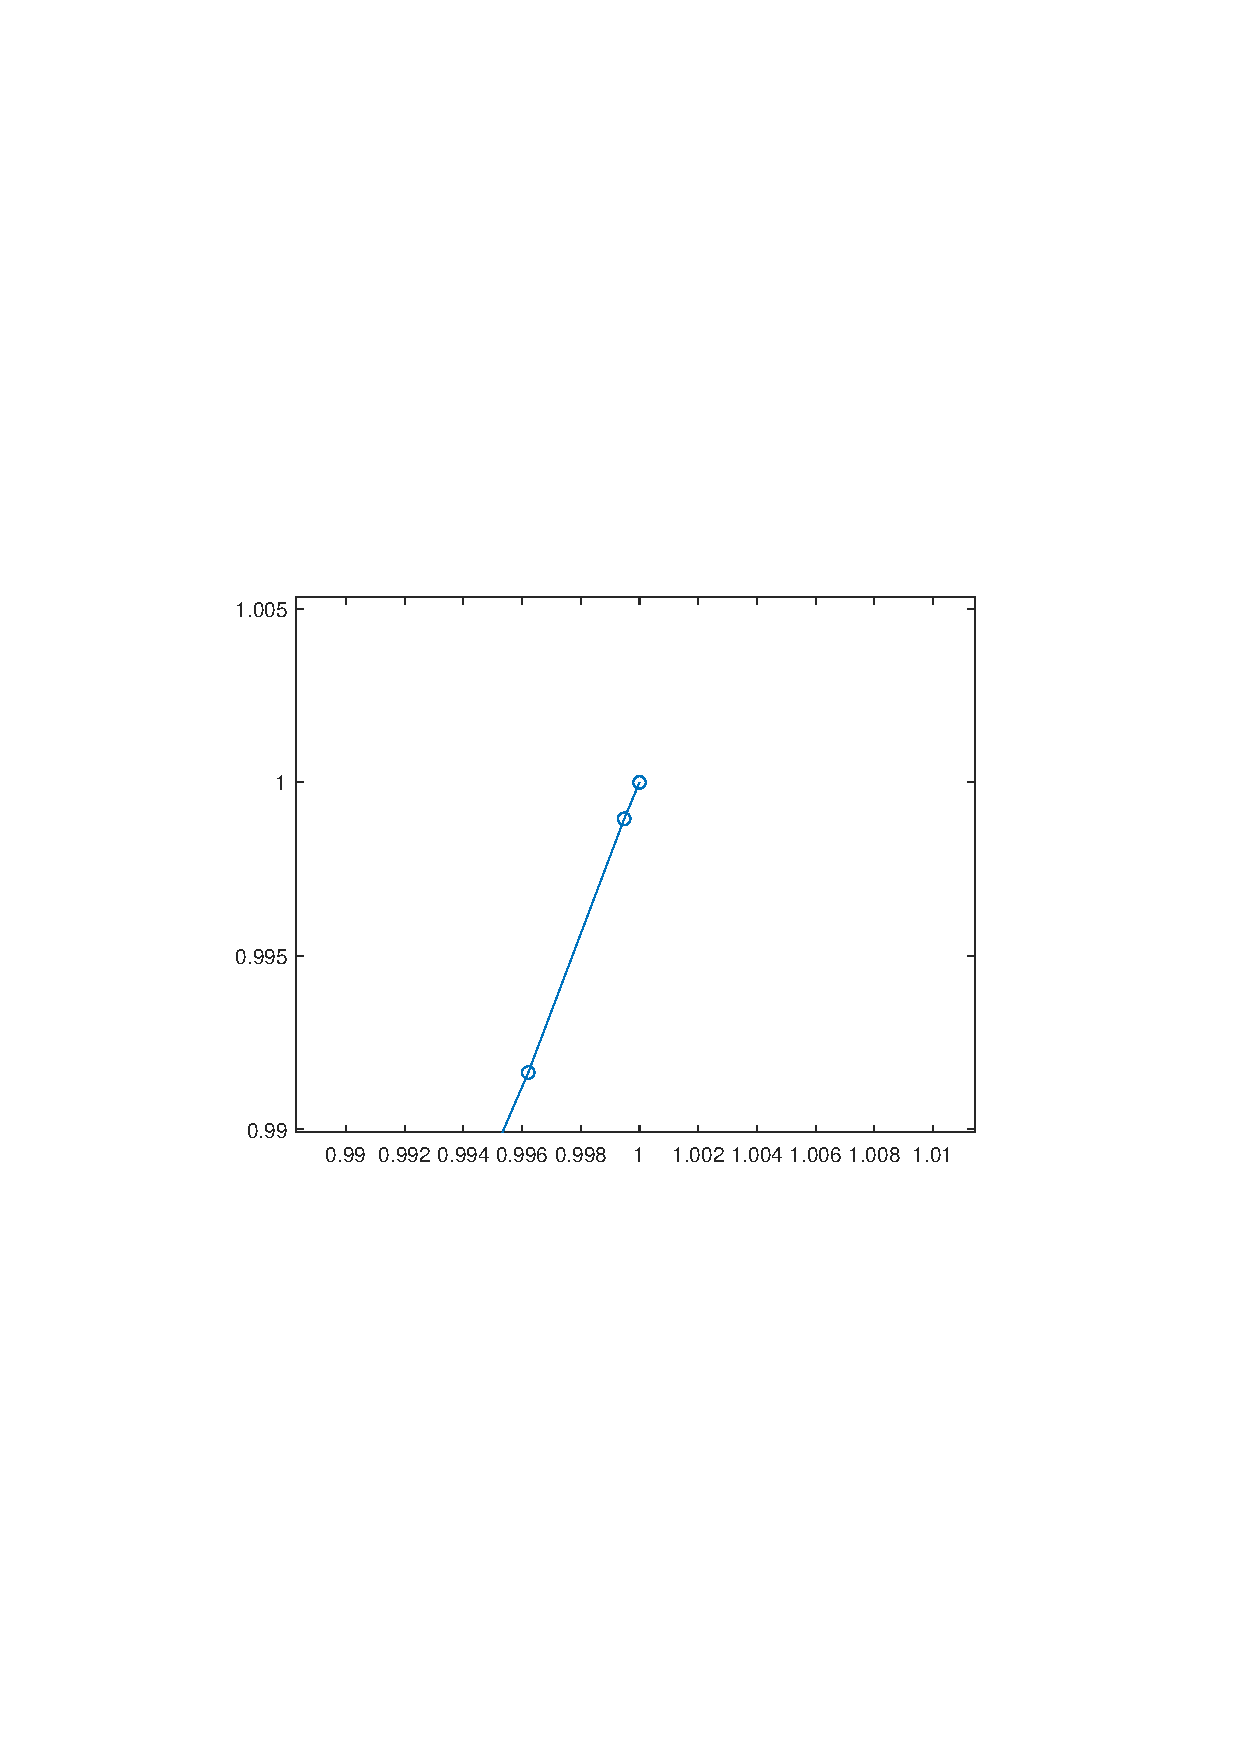
\includegraphics[width=5.3cm]{fig/4_44.pdf}}
\caption{Newton-Armijo in (-1.2,1)}
\label{Fig.lable}
\end{figure}

\begin{lstlisting}
%Result for Newton-Armijo in (-1.2,1)
Step[1]:  x=[ -1.200000 1.000000 ] optim_fx=24.200000
Step[2]:  x=[ -1.175281 1.380674 ] optim_fx=4.731884
Step[3]:  x=[ -0.932981 0.811211 ] optim_fx=4.087399
Step[4]:  x=[ -0.782540 0.589736 ] optim_fx=3.228673
Step[5]:  x=[ -0.459997 0.107563 ] optim_fx=3.213898
Step[6]:  x=[ -0.393046 0.150002 ] optim_fx=1.942585
...
...
...
Step[17]:  x=[ 0.942079 0.881336 ] optim_fx=0.007169
Step[18]:  x=[ 0.967992 0.936337 ] optim_fx=0.001070
Step[19]:  x=[ 0.996210 0.991639 ] optim_fx=0.000078
Step[20]:  x=[ 0.999479 0.998948 ] optim_fx=0.000000
Step[21]:  x=[ 0.999999 0.999998 ] optim_fx=0.000000
Step[22]:  x=[ 1.000000 1.000000 ] optim_fx=0.000000
%牛顿 Armijo 回溯法,,共迭代 22 步
%最优解:
x=[ 1.000000e+00 1.000000e+00 ] optim_fx=0.000000
\end{lstlisting}

\newpage
\subsection{牛顿法总结分析}
在面临梯度变化特别大的情况时,最速下降法显得非常不尽人意,即使在离稳定点非常近的地方依旧不能快速收敛,而是呈锯齿状不断摇摆。由我们所学的知识可以知道,最速下降法的收敛速度强烈依赖于Hessian矩阵的条件数,条件数越高,等值圆越扁,最速下降法的锯齿现象就越明显,这一点可以直观地从图像上看出来。

而牛顿法显得更加“聪明”,因为它利用到了函数的二阶信息,从某种角度来说,最速下降法是将函数在该点用一次函数模型去逼近,然后小心翼翼地迈出一小步,而牛顿法则是在该点用二次函数模型去逼近,然后求解模型函数的极小点,来逼近真正的极小点,这与信赖域法有异曲同工之妙。

\begin{figure}[H]
\centering
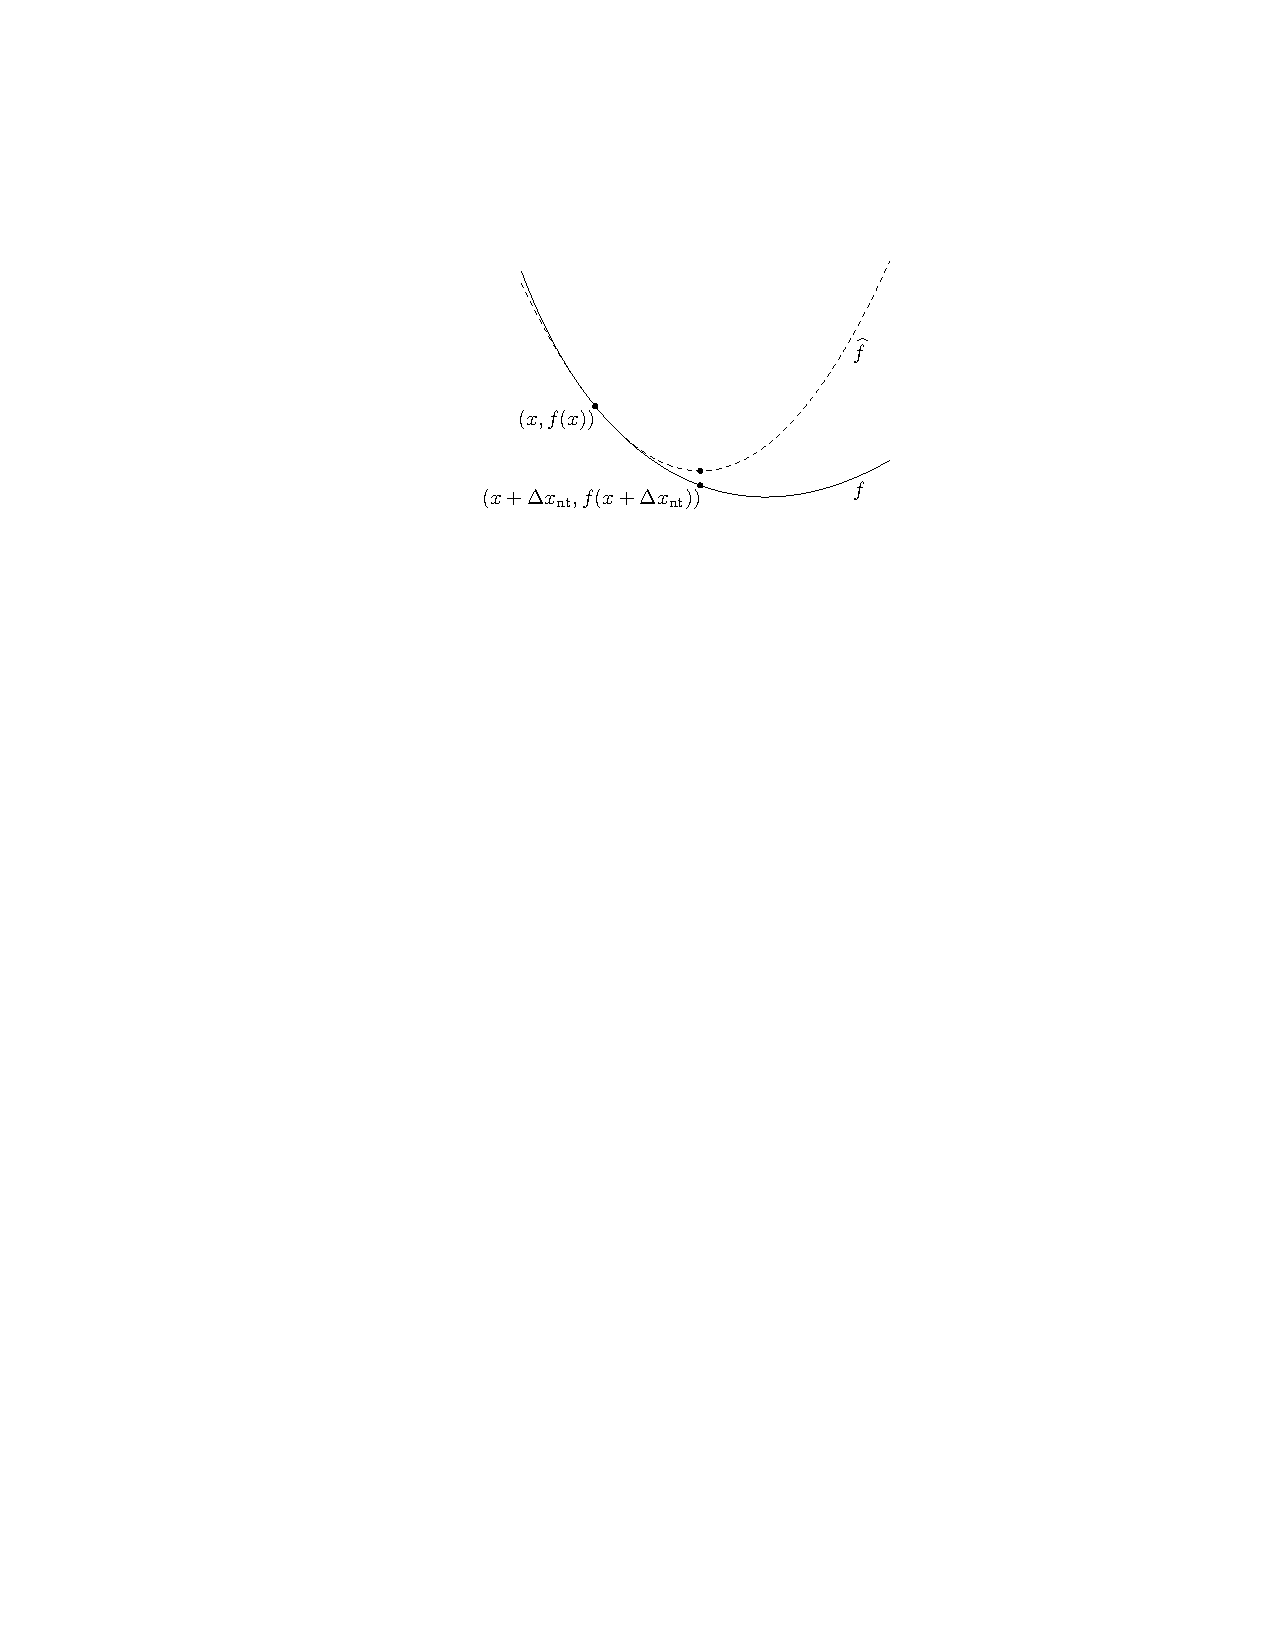
\includegraphics[width=8cm]{fig/4_5.pdf}
\caption{函数$f$\ (实线)和它在$x$处的二阶近似$\hat{f}\ $(虚线)}
\end{figure}

另外,Newton步方向也是在$x$处采用Hessian范数下的的最速下降方向:
\begin{alignat}{2}
\min \quad &\bm{g^Tp} \nonumber\\
\mbox{s.t.}\quad
&\|\bm{p}\|_{\nabla^2f(\bm{x})}=(\bm{p}^T\nabla^2f(\bm{x})\bm{p})^{1/2}=1\nonumber
\end{alignat}

设$\nabla^2f(\bm{x})=\bm{G}$,若$\bm{G}$正定,则可进行Cholesky分解,得$\bm{G}=L^TL$,其中L是上三角矩阵,则原约束条件变为$p^TL^TLp=1\ \Rightarrow \|LP\|_2=1$,设$\bm{v}=LP$,则原优化问题变为:
\begin{alignat}{2}
\min \quad &\bm{g^TL^{-1}v} \nonumber\\
\mbox{s.t.}\quad
&\|\bm{v}\|_2=1\nonumber
\end{alignat}
易得:
\begin{align}
v&=-\dfrac{L^{-1}g}{\|L^{-1}g\|_2}\nonumber\\
p&=L^{-1}v=-\dfrac{{L^TL}^{-1}g}{\|L^{-1}g\|_2}\nonumber\\
&=-\dfrac{G^{-1}g}{\|L^{-1}g\|_2}\nonumber
\end{align}

即$p=-\dfrac{G^{-1}g}{\|L^{-1}g\|_2}$为Newton步方向.

那么,Hessian范数下的的最速下降方向的优越性体现在哪里呢?在这里,我们可以通过坐标变换给出一个有意义的解释:设$\bar{x}=Lx$
\[\|x\|_G=xGx=\|Lx\|_2=\|\bar{x}\|_2\]
故$x$的G—范数就相当于坐标变换后的$\bar{x}$的2—范数
\[\text{定义函数}\bar{f}(\bar{x})=f(L^{-1}\bar{x})=f(x)\]
\[\nabla \bar{f}(\bar{x})=\nabla f(L^{-1}\bar{x})=L^{-T}\nabla f(L^{-1}\bar{x})=L^{-T}\nabla f(x)\]
那么在变换坐标系下沿$\bar{f}$的最速下降方向为$-L^{-T}\nabla f(x)$,换回原坐标系后的方向为$-L^{-1}(L^{-T}\nabla f(x))=-G^{-1}\nabla f(x)$,即Newton步方向
\[\nabla^2 \bar{f}(\bar{x})=\nabla^2 
f(L^{-1}\bar{x})=L^{-T}\nabla^2f(x)L^{-1}\]
那么在变换坐标系下沿$\bar{f}$的Hessian阵为\[L^{-T}GL^{-1}=L^{-T}L^TLL^{-1}=\bm{I}\]

其几何意义就是先在$x$点处根据其Hessian阵进行坐标变换,将原来的椭圆等值线变换为标准的圆形等值线,即变换后的Hessian阵为单位阵,在此基础上进行最速下降法,由于等值线是标准的圆形,因此一次梯度下降就能抵达圆心,即迭代到了二次模型函数的最小点.